% !TEX root = main.tex
\setlength{\parskip}{.5mm plus 0mm minus 0mm}
\chapter{Theoretical framework}
Quantum computing is based on a general framework that does not depend on the particular physical quantum platform. In this chapter, important concepts such as qubits and quantum operations are described from a theoretical point of view, before showing how we can realize them with trapped ions. The same goes with quantum networking, the concept and the realization can be treated separately and they will be described in this chapter. Next, key properties of Gaussian beams are presented: the beam shapes emitted by our lasers. Acousto-optical interactions are then introduced and studied to give an idea of how AODs work and how they can be used to steer a laser beam. Lastly, a brief overview of two key experiments is given.

\section{Quantum logic with trapped ions}
\subsection{Quantum computer and quantum gates}
\label{sec:quantumoperations}
The concepts of quantum computing are borrowed and extended from classical computation. In the classical case, information is mostly represented in terms of binary digits, the so called bit, essentially mapping information to a base-2 number. Information processing is done with gates acting of those numbers. The idea of a quantum computer is still to encode information in a binary form, but due to the nature of quantum mechanics, a quantum bit (in short qubit) gains new features that can be exploited to perform different kind of operations.\par
A qubit is formally a normalized wave function that can be written as a superposition of two orthogonal states indicated usually with $\ket{0}$ and $\ket{1}$:
\begin{equation}
\label{qubit}
\ket{\psi} = \alpha \ket{0} + \beta\ket{1},
\end{equation}
where $\alpha,\beta$ are probability amplitudes, i.e. two complex numbers that satisfy the relationship $|\alpha|^2+|\beta|^2 = 1$. The outcome of measuring a qubit in the logical basis (outcomes 0 or 1) will give the value 0 with a probability of $|\alpha|^2$ and 1 with a probability of $|\beta^2|$.\par
Qubits also have a geometrical representation that can be useful. Equation \eqref{qubit} depends on 4 real numbers, however since $\psi$ is normalized, we can rewrite the expression as \cite{chuang}
\begin{equation}
\ket{\psi} = e^{i\gamma}\left(\cos\frac{\theta}{2}\ket{0} + e^{i\varphi}\sin\frac{\theta}{2}\ket{1}\right).
\end{equation}
The global phase factor $e^{i\gamma}$ can be left out as it does not influence the measurement outcome, leaving only two real numbers: $\theta$ and $\varphi$. A qubit can therefore be represented geometrically with normalized spherical coordinates. The so called Bloch sphere is depicted in Figure \ref{blochsphere}, every point on its surface represents a different state of the qubit. Qubit manipulation can be visualized as trajectories on the surface. The drawback of this representation is that it is limited to only one qubit, so it loses usefulness when dealing with multiple qubits.
\begin{figure}[H]
\centering
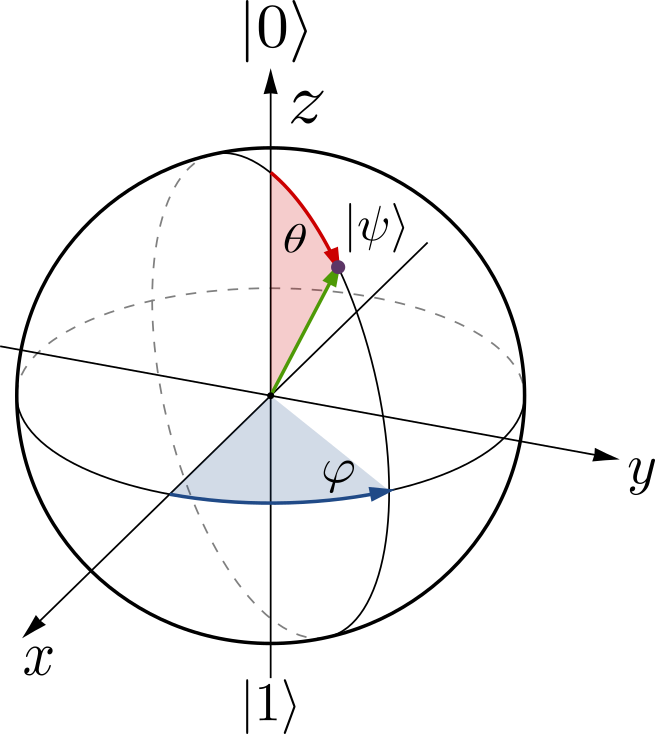
\includegraphics[width = .4\textwidth]{bloch_sphere}
\caption{The Bloch sphere. The states $\ket{0}$ and $\ket{1}$ are at the poles of the sphere, every other point of the surface represents a superpositions of these states. A single qubit quantum gate can be seen as trajectory on the surface mapping one state to another.}
\label{blochsphere}
\end{figure}

An alternative way of dealing with qubits is via vectors and matrices. We can assign to the states $\ket{0}$ and $\ket{1}$ the following:
\begin{equation}
\ket{0} = \begin{pmatrix}
 1 \\
 0
\end{pmatrix} \quad
\ket{1} = \begin{pmatrix}
 0 \\
 1
\end{pmatrix} \implies \ket{\psi} = \begin{pmatrix}
 \alpha \\
 \beta
\end{pmatrix}.
\end{equation}
In this representation, single qubit rotations are calculated using $2\times2$ unitary matrices. These kind of operations are named \emph{quantum gates} and they are the building blocks of quantum computing. Quantum algorithms can be written as a sequence of quantum gates. For a single qubit, any gate can be written as multiple combination of two operations, e.g. \cite{hempel}
\begin{equation}
\label{quantumgates}
U_z(\Theta) =  \begin{pmatrix}
 e^{-i\frac{\Theta}{2}} & 0 \\
 0 & e^{i\frac{\Theta}{2}}
\end{pmatrix} \qquad U_\varphi(\theta) = \begin{pmatrix}
\cos\frac{\theta}{2} & -i e^{-i\varphi}\sin\frac{\theta}{2} \\
-ie^{i\varphi}\sin\frac{\theta}{2} & \cos\frac{\theta}{2}
\end{pmatrix}.
\end{equation}
These two matrices can be seen as two different rotations in the Bloch sphere, $U_z$ is a rotation around the $z$ axis by the angle $\Theta$, while $U_\varphi$ is a rotation around an axis located in the x-y plane. Important examples of single qubit gates are the Hadamard gate $H$, which creates a superposition of one qubit starting from the state $\ket{0}$, or $\ket{1}$, and the phase shift gate $R_\phi$ that shifts the phase:
\begin{equation}
\label{Hadamard}
 H = \frac{1}{\sqrt{2}}\begin{pmatrix}
 1  & 1\\
1 & -1
 \end{pmatrix} \equiv U_{\varphi=\pi}\left(\frac{\pi}{2}\right)U_z(\pi) \qquad R_\phi = \begin{pmatrix}
 1  & 0\\
0 & e^{i\phi}
 \end{pmatrix} \equiv e^{i\varphi/2}U_z(\varphi).
\end{equation}
% As we have seen, a single qubit has already the advantage of superposition compared to classical case. When considering multiple qubits, we gain even more quantum mechanical features like entanglement. This phenomenon does not have a classical analogy and it is an extremely useful tool in quantum information. Let us consider only 2 qubits, a particular case would be
% \begin{equation}
% \ket{\psi} = \frac{1}{\sqrt{2}}\left(\ket{00} + \ket{11}\right).
% \end{equation}
% If a measurement is made on one of the two qubit and, for instance, the outcome is 0, the outcome of a measurement on the second qubit  will be 0 with unit probability. Viceversa, if the outcome of the first measurement was 1, the outcome of the second measurement is always 1.\\
Gates that involve $N$ qubits are written as $2^N\times 2^N$ unitary matrices, a famous example is the controlled not (CNOT) gate
\begin{equation}
\text{CNOT} = \begin{pmatrix}
1  & 0 & 0 & 0\\
0 & 1 & 0 & 0\\
0 & 0& 0 & 1 \\
0 & 0 & 1 &0
\end{pmatrix}.
\end{equation}
Which can be used to generate entanglement between two qubits. It can be shown \cite{chuang} that the examples of this section: $H$ gate, phase gate, and CNOT gate form a universal set of quantum gates, i.e. a sequence of these gates approximates every other possible unitary quantum operation.

\subsection{Ion qubits and laser-ion interactions}
\label{laserioninteractions}
Qubits can be encoded in any pair of orthogonal quantum states of a physical system. %REWRITE (In the case of an ion it is possible to take two internal electronic states, the qubit is then implemented in their transition. In figure \ref{qubitschemereference} the level scheme of $^{40}\text{Ca}^+$ is presented. The lifetime of the excited level has to be long enough to carry out all the quantum operations without spontaneous scattering. A common choice is the transition $\ket{\text{S}_{1/2}} \to \ket{\text{D}_{5/2}}$, where the ground state $\ket{\text{S}_{1/2}}$ represents the state $\ket{0}$ and the excited state $\ket{\text{D}_{5/2}}$ will be $\ket{1}$).
In Figure \ref{qubitschemereference} the level scheme of $^{40}\text{Ca}^+$ is presented. The states $\ket{\text{S}_{1/2}}$ and $\ket{\text{D}_{5/2}}$ are a common choice to encode a qubit. The ground state $\ket{\text{S}_{1/2}}$ represents the state $\ket{0}$ and the long lived ($\sim$ 1 s) excited state $\ket{\text{D}_{5/2}}$ can be $\ket{1}$. As these levels are directly connected by an electric-quadrupole transition at an optical wavelength (729 nm), this kind of qubit is often referred to as an optical qubit.
Lasers provide a way to directly manipulate the population of these two levels and therefore to manipulate the state of the qubit.\par
The laser set up in this thesis is the 393 nm, which interacts via a dipole transition (different from the 729 nm transition) with the atomic ion, we model therefore the atom-light interactions as dipole interaction. In the case of a quadrupole interaction, the equations below still hold with the exception of the Rabi frequency, which will no longer depend linearly with the electric field. For a proper treatment of the quadrupole interaction see \cite{ross}.\par
%The interaction between ion and laser is now presented using a simple model: a two-level atom with dipole interaction with the laser field.
Consider the simple two-level system in Figure \ref{2levelatom}, where the states $\ket{0}$ and $\ket{1}$ are separated by a frequency $\omega_0$, while the laser is assumed to be monochromatic with frequency $\omega_l$. The difference $\Delta = \omega_l -\omega_0$ is called detuning and we assume to be in the near-resonant regime $\Delta \ll \omega_0$. % The laser light in this case can be described classicaly in the dipole approximation.
%This assumption can be explained as follow, the wavelength of transitions in an atom, are typically in the optical regime: hundreds of nanometers, which is order of magnitude greater then the typical atom dimension. Thus, the electric field can be considered constant over the atom size. This allows to expand the electric field in Taylor series and remove every spatial dependent term in the so called dipole approximation.
The Hamiltonian of the atomic part can be written as:
\begin{equation}
H_a = \hbar\omega_0 \ket{1}\bra{1},
\end{equation}
where $\omega_0$ is the frequency difference between the ground and excited state, the energy of the ground state has also been set to 0.
\begin{figure}
\centering
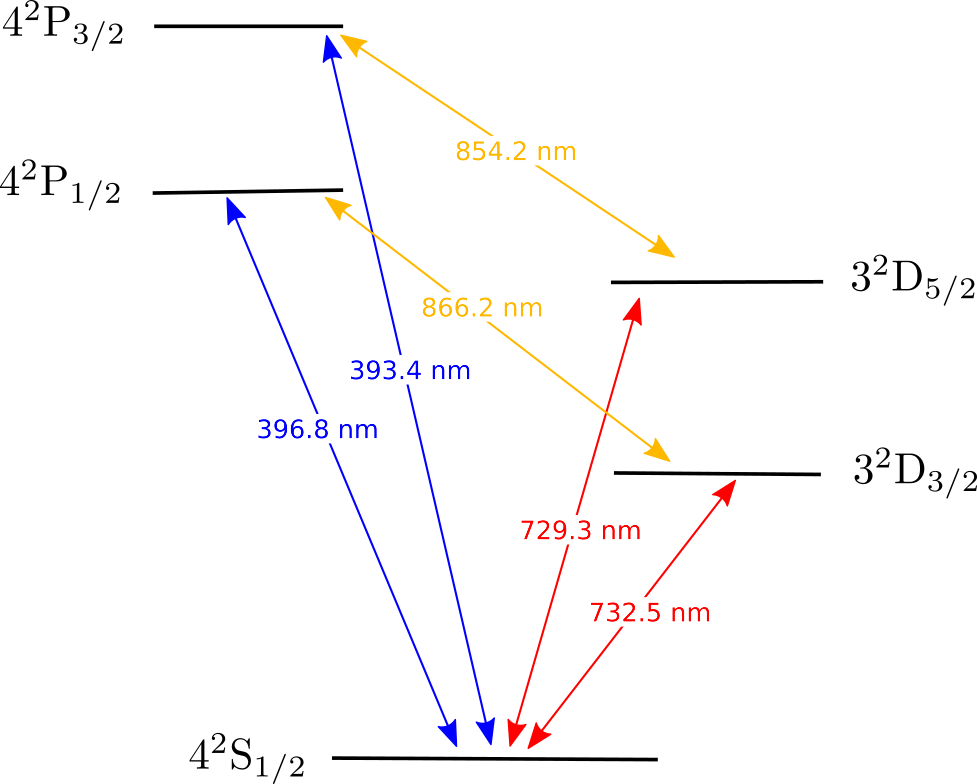
\includegraphics[width = .6 \textwidth]{calciumscheme}
\caption{Level scheme of $^{40}\text{Ca}^+$, notation is $n^{2s+1}l_{j,m_j}$, where $n$ is the principal quantum number, $s$ the electron spin, $l$ the orbital angular moment, $j = |l\pm s|$ the total angular moment, and $m_j$ the magnetic quantum number. Detailed description is in Section \ref{sec:calciumion}. For quantum computing purposes, the chosen qubit transition is the long lived quadropole transition $\ket{\text{S}_{1/2}} \to \ket{\text{D}_{5/2}}$ at 729 nm between a single pair of Zeeman states ($m_j$). Blue and orange transitions are dipole transitions suitable for cooling, and imaging. Red transitions are dipole forbidden, but accessible via electric quadrupole, they are used to encode qubits. In addition, the 854 nm transition is tuned in resonance with the cavity for photon generation purposes.}
\label{qubitschemereference}
\end{figure}
The Hamiltonian of the interaction between the dipole atomic moment $\mathbf{d}$ and the electric field of the laser can be written \cite{steck}
\begin{equation}
H_{int} = -\mathbf{d}\cdot \mathbf{E}
\end{equation}
where the electric field of the laser  will be treated classically and the dipole approximation is assumed. This means
\begin{equation}
\mathbf{E}(t) = \hat{\mathbf{\varepsilon}} E_0 \cos(\omega_l t+\varphi) = \hat{\mathbf{\varepsilon}} \frac{E_0}{2} \left(e^{-i(\omega_l t+\varphi)} + e^{i(\omega_l t+\varphi)}\right),
\end{equation}
where $\hat{\varepsilon}$ is the unit polarization vector, and $\varphi$ is the laser phase at the point of the ion at time 0. The next step is to work out the dipole operator, this can be done by applying the identity $\ket{0}\bra{0} + \ket{1}\bra{1}$ on both sides of $\mathbf{d}$. Due to parity arguments \cite{steck}, only the non diagonal terms are non-vanishing, giving
\begin{equation}
\mathbf{d} = \braket{0|\mathbf{d}|1}\left(\ket{0}\bra{1} + \ket{1}\bra{0}\right) \equiv \braket{0|\mathbf{d}|1}(\sigma + \sigma^\dagger).
\end{equation}
Combining the last three equations yields
\begin{equation}
\label{eq:hint}
H_{int} = - \braket{0|\hat{\varepsilon} \mathbf{d}|1}\frac{E_0}{2}(\sigma e^{i(\omega_l t+\varphi)} + \sigma^\dagger e^{-i(\omega_l t+\varphi)} + \sigma e^{-i(\omega_l t+\varphi)} + \sigma^\dagger e^{i(\omega_l t+\varphi)})
\end{equation}
A rotating wave approximation is used now: in the interaction picture, the operator $\sigma$ ($\sigma^\dagger$) evolves under the Hamiltonian $H_a$ in time as $\widetilde{\sigma} = e^{i H_a t/\hbar}\sigma e^{-i H_a t/\hbar} = \sigma e^{-i\omega_0 t}$ ($\widetilde{\sigma}^\dagger=\sigma^\dagger e^{i\omega_0 t}$). Therefore, Equation \ref{eq:hint} in the interaction picture contains terms that oscillate as $\propto e^{\pm i(\omega_l-\omega_0 )t}$, and $\propto e^{\pm i(\omega_l+\omega_0 )t}$. We can drop the fast oscillating terms and keeping only those that depend on time as $\propto e^{\pm i(\omega_l-\omega_0 )t}$. The validity of this approximation is given by the fact that $\omega$ and $\omega_0$ are in the optical regime, thus they oscillate extremely fast and average to zero, the interesting slow dynamic is given only by their difference: the detuning.
Going back in the Schrödinger picture yields the final form of the interaction Hamiltonian
\begin{equation}
H_{int} = \frac{\hbar \Omega}{2}(\sigma e^{i(\omega_l t+\varphi)} + \sigma^\dagger e^{-i(\omega_l t+\varphi)}),
\end{equation}
 where we defined the Rabi frequency $\Omega \equiv - \braket{0|\hat{\varepsilon} \mathbf{d}|1}E_0/\hbar$. The Rabi frequency depends linearly with the applied electrical field and hence its square is proportional to the intensity of the laser $\Omega ^2 \propto I$. To summarize, the total system Hamiltonian is
 \begin{equation}
 \label{2levelatomhamiltonian}
H = H_a + H_{int} = \hbar\omega_0 \ket{1}\bra{1} + \frac{\hbar \Omega}{2}(\sigma e^{i(\omega_l t+\varphi)} + \sigma^\dagger e^{-i(\omega_l t+\varphi)}).
 \end{equation}
To eliminate the time dependence, we can go in the rotating frame with the unitary transformation $U = e^{i\omega_l t \ket{1}\bra{1}}$, the Hamiltonian in this frame is
\begin{equation}
\label{Hamiltonianrotatingframe}
\widetilde{H} = -\hbar \Delta \ket{1}\bra{1} + \frac{\hbar \Omega}{2}(e^{i\varphi}\sigma + e^{-i\varphi}\sigma^\dagger)
\end{equation}
\begin{figure}
\centering
\includegraphics[width = .4\textwidth]{2levelatom}
\caption{2-level atom scheme, the ground and excited states are denoted as $\ket{0}$, and $\ket{1}$. $\omega_l$ is the laser frequency, which is detuned by $\Delta \equiv \omega_l - \omega_0$ from the transition frequency $\omega_0$.}
\label{2levelatom}
\end{figure}
The time dependence is now gone, and the unitary evolution matrix can be calculated as
\begin{equation}
\label{laserpulse}
U(t) = \exp\left\{-\frac{i}{\hbar} \widetilde{H} t \right\} =
 \begin{pmatrix}
  \cos\left(\frac{\widetilde{\Omega} t}{2}\right) + i \frac{\Delta}{\widetilde{\Omega}} \sin\left(\frac{\widetilde{\Omega} t}{2}\right) & -ie^{i\varphi}\frac{\Omega}{\widetilde{\Omega}}  \sin\left(\frac{\widetilde{\Omega} t}{2}\right) \\
  -ie^{-i\varphi}\frac{\Omega}{\widetilde{\Omega}}  \sin\left(\frac{\widetilde{\Omega} t}{2}\right)  & \cos\left(\frac{\widetilde{\Omega} t}{2}\right) - i \frac{\Delta}{\widetilde{\Omega}} \sin\left(\frac{\widetilde{\Omega} t}{2}\right)
\end{pmatrix}.
\end{equation}
Where $\widetilde{\Omega} = \sqrt{\Delta^2 + \Omega^2}$ is the generalized Rabi frequency. In the case of zero detuning ($\Delta = 0$) the matrix is the same as Equation \eqref{quantumgates}, thus a resonant laser pulse implements the qubit rotation $U_{\varphi}(\theta)$.\par
As an example, let us take the atom in the ground state $\ket{\psi} = \ket{0}$ and apply the unitary evolution \eqref{laserpulse}. The probability to be in the excited state becomes
\begin{equation}
\label{eq:rabifrequency}
\mathbb{P}\{\ket{1}\}(t) = |\braket{1|U(t)|0}|^2 = \frac{\Omega^2}{\Omega^2+\Delta^2} \sin^2\left(\frac{\widetilde{\Omega}t}{2} \right)
\end{equation}
This equation is plotted in Figure \ref{rabiflops}. For $\Delta = 0$, we get a cosine behaviour, the so called Rabi oscillations. The probability amplitude for the electron, under continuous drive by a laser, will oscillate between the ground and excited state at a frequency $\Omega/2$. Detuning damps the amplitude of such oscillations and increases the oscillation frequency. Rabi oscillations are an important tool in quantum information, laser pulses can prepare the state of the qubit in any superposition, e.g. starting in the $\ket{0}$ state, a $\pi/2$ pulse ($\Omega t = \pi/2$ and phase $\varphi=0$) will result in the state $(\ket{0} - i\ket{1})/\sqrt{2}$, with a $\pi$ pulse ($\Omega t = \pi$, $\varphi=\pi$) the population is completely transferred to another level $\ket{0}\to \ket{1}$. These pulses can be used to implement e.g. the Hadamard gate of Equation \eqref{Hadamard}.
\begin{figure}[H]
\centering
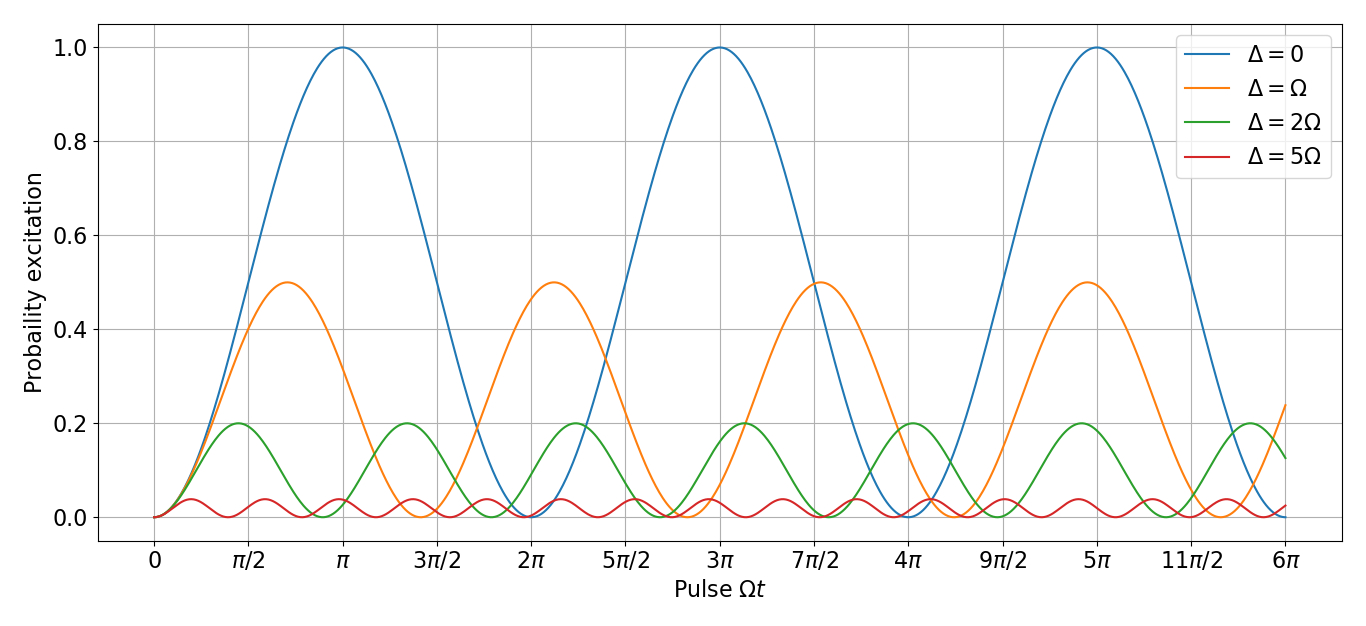
\includegraphics[width = 1\textwidth]{rabiflops}
\caption{Rabi flops for different detunings $\Delta$, starting from the $\ket{0}$ state. Equation \eqref{eq:rabifrequency}.}
\label{rabiflops}
\end{figure}
As the light is detuned from the transition, Rabi oscillations are suppressed: the amplitude is reduced by a factor of 0.5 already with $\Delta = \Omega$, while a factor of 10 in reduction is achieved with a detuning of $\Delta = 5\Omega$. However, another effect occurs in the off-resonant regime, the energy levels are shifted.
The shift $\delta$ can be calculated by finding the eigenvalues of the Hamiltonian \eqref{Hamiltonianrotatingframe}, which can be written in matrix form and diagonalized. We find that there are two eigenstates $\ket{+}$ and $\ket{-}$ called dressed states with eigenvalues
\begin{equation}
E_{\pm} = -\frac{\hbar\Delta}{2} \pm \frac{\hbar}{2}\sqrt{\Delta^2 +\Omega^2}.
\end{equation}
In the limit $\Delta \gg \Omega$, dressed states tend to the bare states $\ket{+} \to \ket{1},\ket{-}\to \ket{0}$, and the energies become
\begin{equation}
\label{eq:starkshift}
E_{\pm} \to -\frac{\hbar \Omega}{2} \pm \frac{\hbar \Omega}{2} \pm \frac{\hbar \Omega^2}{4\Delta} \implies \delta = \pm\frac{\Omega^2}{4\Delta}.
\end{equation}
The effective Hamiltonian for the off-resonant regime can be derived following a Markovian approximation \cite{acstarkhamiltonian}
\begin{equation}
H_{AC} = \frac{1}{\hbar \Delta} [\sigma,\sigma^\dagger] = \frac{\hbar \delta}{2}\sigma_z
\end{equation}
The corresponding evolution is
\begin{equation}
\label{acstarkrotation}
U(t) = \exp\left\{-\frac{i}{\hbar} H_{AC} t \right\} =
 \begin{pmatrix}
   \exp\left\{i\frac{\delta}{2}t\right\} & 0\\
   0 & \exp\left\{i\frac{\delta}{2}t\right\}
\end{pmatrix}.
\end{equation}
This matrix implements the quantum gate $U_z(\Theta)$ from Equation \eqref{quantumgates}.


\subsubsection{Three-level model}
\label{sec:threelevel}
\begin{figure}
\centering
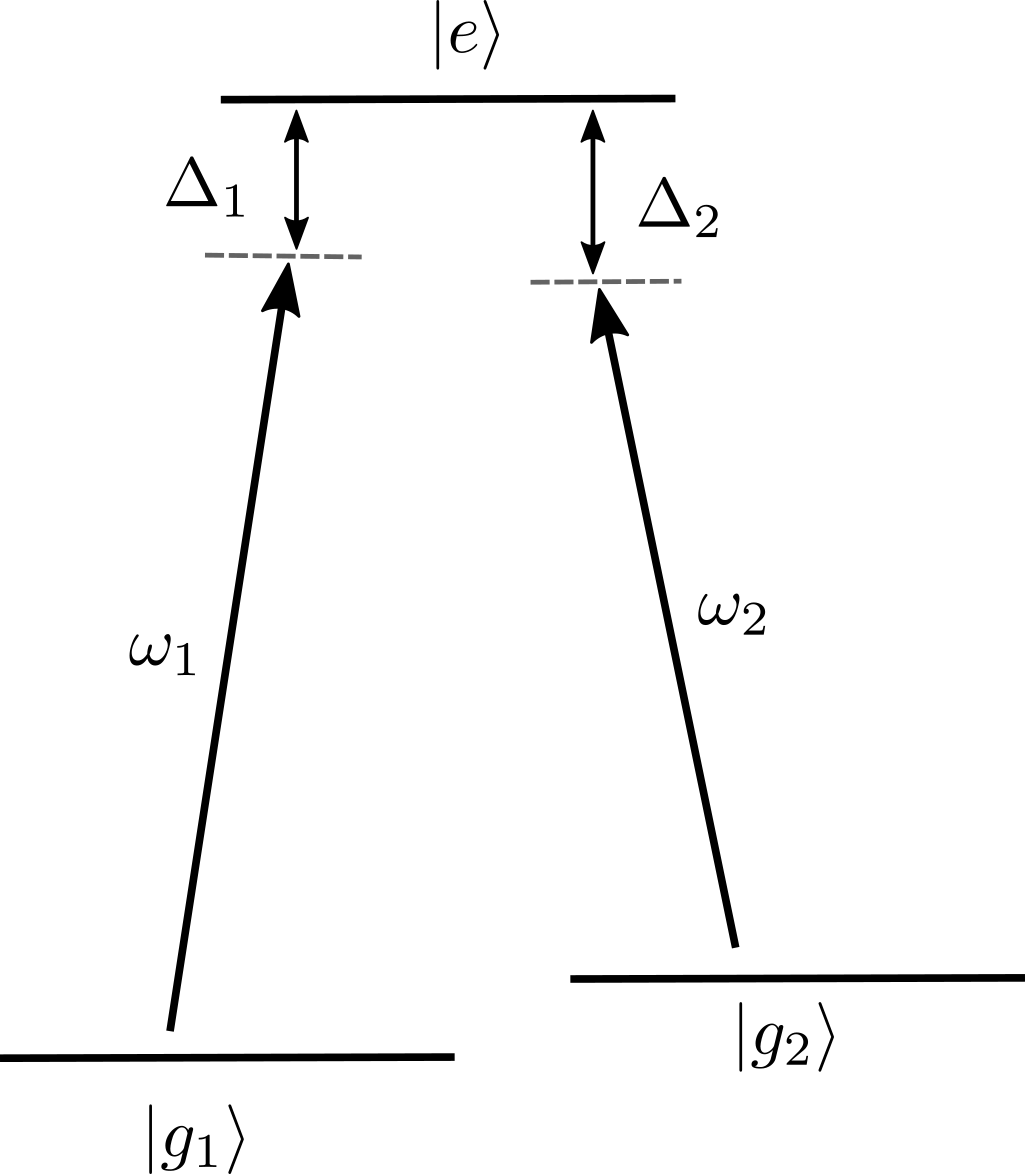
\includegraphics[width = .3\textwidth]{3levelmodel}
\caption{3 level atom model. Two long lived ground states $\ket{g_1}$, $\ket{g_2}$ couple to an excited level $\ket{e}$ (atomic frequencies $\omega_{1e}$, and $\omega_{2e}$ respectively) through two lasers of frequencies $\omega_1$, $\omega_2$ detuned respectively $\Delta_1,\Delta_2$ from the transitions.}
\label{3levelmodel}
\end{figure}
We extend our model to a 3 level $\Lambda$ type atom driven by two lasers, which more closely resembles the real experimental situation (393 nm, 729 nm lasers and $\ket{\text{S}_{1/2}},\ket{\text{P}_{3/2}},\ket{\text{S}_{5/2}}$ states, see Figure \ref{qubitschemereference}) in the experiments in this thesis. The model contains new effects that explain photon generation and qubit gates. In particular, stimulated Raman transition will be discussed, and we will show how, under certain conditions, the system can be approximated as an effective 2 level atom. The system is depicted in Figure \ref{3levelmodel}, two ground states $\ket{g_1}$ and $\ket{g_2}$ are present together with a common excited state $\ket{e}$. Two different lasers $\omega_1,\omega_2$ drive the transition $\ket{g_1} \to \ket{e}$ and $\ket{g_2} \to \ket{e}$, where the atomic frequencies are $\omega_{1e}$, and $\omega_{2e}$ respectively. Detunings are defined as $\Delta_1 = \omega_1 - \omega_{1e}$ and $\Delta_2 = \omega_2 - \omega_{2e}$. In the case of calcium, the ground states are $\ket{\text{S}_{1/2}}$, and $\ket{\text{D}_{5/2}}$. This is the qubit transition, and it is long lived ($\sim 1$ s), such that any spontaneous emission from D to S can be neglected. The excited level is $\ket{\text{P}_{3/2}}$ which can decay into both ground states with branch ratio of 94\% from P$\to$S ($\sim$ 7.4 ns) and 5.3\% from P$\to$D ($\sim 101$ ns), we neglet decay to the $\ket{\text{D}_{3/2}}$ state.\par
%In this model we assume that each laser light couples only to one transition and that . %the two ground states are not separated by an optical frequency $\omega_{2e} - \omega_{1e} \ll \omega_1,\omega_2$, and that the detunings are nearly equal $\Delta_1 \simeq \Delta_2$. As a consequence, each laser light couples only to one transition.\\
Following the approach of \cite{steck}, the bare atom Hamiltonian is
\begin{equation}
H_a = -\hbar \omega_{1e}\ket{g_1}\bra{g_1} - \hbar \omega_{2e}\ket{g_2}\bra{g_2},
\end{equation}
with the convention of setting the excited level energy to 0. The electric field is now the sum of the two laser fields
\begin{equation}
\mathbf{E}(t) = \hat{\varepsilon_{01}} E_{01} \cos(\omega_{1} t \varphi_1) + \hat{\varepsilon_{02}} E_{02} \cos(\omega_2 t + \varphi_2).
\end{equation}
As in Section \ref{laserioninteractions}, we then consider a dipole interaction, make the dipole approximation and a rotating wave approximation. Finally, the full final Hamiltonian in the rotating frame is
\begin{equation}
H = \hbar \Delta_1 \ket{g_1}\bra{g_1} + \hbar\Delta_2 \ket{g_2}\bra{g_2}+ \frac{\hbar \Omega_1}{2}\left(\sigma_1 e^{i\varphi_1} +\sigma_1^\dagger e^{i\varphi_1}\right)+ \frac{\hbar \Omega_2}{2}\left(\sigma_2 e^{i\varphi_2} +\sigma_2^\dagger e^{i\varphi_2}\right),
\end{equation}
where $\Omega_i = -\frac{\braket{g_1|\varepsilon_i \cdot \mathbf{d}|e}E_{i}}{\hbar}$, and $\sigma_i = \ket{g_i}\bra{e}$. Under certain conditions, this Hamiltonian describes a Raman process, where state population is transferred coherently between $\ket{g_1}$ and $\ket{g_2}$. Specifically, the Raman conditions are: equal detunings $\Delta_1 = \Delta_2 \equiv \Delta$ (Raman resonance), and $\Delta \gg \Omega_1,\Omega_2$.
Intuitively, this corresponds to the situation where the difference of the two driving frequencies $(\omega_1-\omega_2)$ is equal to the frequency splitting between $\ket{g_1}$, and $\ket{g_2}$.\par
Following \cite{russo} it can be shown that, under the previous conditions, the Raman process leads to an effective coupling directly between the two ground states. The effective Rabi frequency of the coherent population transfer $\ket{g_1} \to \ket{g_2}$ is \cite{steck}
\begin{equation}
\label{eq:effectiverabi}
\Omega_{eff} = \frac{\Omega_1\Omega_2}{2\Delta}.
\end{equation}

\subsubsection{Dissipative processes}
\label{sec:dissipation}
In our experiments spontaneous emission can play a role as the condition $\Delta \gg \Omega_1,\Omega_2$ is only partially fulfilled. In this section therefore, we present a quantitative overview of spontaneous scattering as a function of detuning and Rabi frequency of each laser. Dissipative processes do not follow a Hermitian evolution, hence their mathematical description is done heuristically by adding terms in the Heisenberg equation
\begin{equation}
\label{masterequation}
\frac{d\rho}{dt} = \frac{1}{i\hbar}[H,\rho] + \mathcal{L}(\rho).
\end{equation}
This equation is usually referred to as master equation in Lindblad form, where $\rho$ is the density matrix of the system. The superoperator
$\mathcal{L}(\rho)$ contains phenomena not included in the Hamiltonian. For spontaneous emission, the form of $\mathcal{L}(\rho)$ is \cite{quantumnoise}
\begin{equation}
\mathcal{L}(\rho) = \frac{\Gamma}{2}(2\sigma \rho \sigma^\dagger -\sigma^\dagger\sigma \rho - \rho \sigma^\dagger \sigma),
\end{equation}
where $\Gamma$ is the spontaneous emission rate.
% The master equation \eqref{masterequation} can be explicitly written for every component of the density matrix $\rho$,
%in the rotating frame they are called optical Bloch equations. The solution for the excited population in the case of the 2 level atom shows that the effect of spontaneous emission is to damp Rabi oscillations.
For the three level atom, in the effective 2 level system picture, the spontaneous emission is modified as \cite{russo}
\begin{equation}
\label{eq:gammaeff}
\Gamma_{eff} = \left(\frac{\Omega_1}{2 \Delta_1}\right)^2 \cdot \Gamma.
\end{equation}
The ratio between $\Gamma_{eff}$ and the AC Stark shift \eqref{eq:starkshift} $\delta/\Gamma_{eff}\propto \Delta$ dictates which effect is dominant, i.e. by increasing the detuning, the effective rate of spontaneous scattering can be reduced in favor of the AC Stark shift. This regime can be used to implement a phase gate where the qubit is encoded in the $\ket{g_1}\to\ket{g_2}$ transition and the phase of $\ket{g_1}$ is manipulated by Stark shifting the transition $\ket{g_1}\to \ket{e}$. In the experiment of Section \ref{sec:singlequbitmanipulation}, we implement this gate on a single ion in a string.


\section{Quantum networking with trapped ions}
\subsection{General introduction}
A quantum network is a collection of quantum processors, referred to as nodes, interconnected with quantum channels, referred to as links. Nodes are used for processing and storing quantum information, while links for quantum information distribution \cite{kimble}. Links are typically realized with traveling photons, either in free-space \cite{Hughes2002} or in optical fibers. Nodes can be realized using different physical systems: trapped ions \cite{ion_quantumnetwork}, neutral atoms \cite{Ritter2012}, atomic ensembles \cite{kimble}. Nodes and links are connected through an interface that converts a stationary qubit in a node to a flying qubit over the network.  In the next section we will explore how such an interface can be realized by placing an ion-qubit in an optical cavity.\par
Faithful transmission of quantum states over long distances can be a daunting problem as quantum information cannot be cloned \cite{nocloning} and noisy channels can destroy the delicate nature of qubits. Quantum repeaters have been designed \cite{quantumrepeters} to circumvent these problems through a series of protocols which include entanglement purification: a form of error correction \cite{Pan2001}. Once entanglement has been established between nodes, other network functionalities become available, like for instance teleportation \cite{PhysRevLett.70.1895}. Entanglement generation, and quantum repeaters are just some examples of the fundamental steps necessary for building a quantum network, for a more in depth review look at \cite{Wehnereaam9288}.


\subsection{Cavity QED}
\label{sec:cavityqed}
A single trapped ion is a single photon source and those photons can be collected either with a lens \cite{ion_quantumnetwork}, with mirrors \cite{PhysRevLett.120.193603} or with optical cavities \cite{Keller2004bis}. Photon collection from ions using an optical cavity is a powerful approach, that will now be introduced in detail. A cavity placed around ions can improve the efficiency of photon collection as the probability of a photon to be emitted in the cavity mode is enhanced with respect to emitting in free space \cite{Kimble_1998}.\par
In this Section a simple model of a two-level system in a cavity is described following the approach of \cite{steck}. We described the cavity electric field as quantized, with $a,a^\dagger$ the creation and annihilation operators of a single photon in the cavity mode, respectively.
The quantized electric field assumes the form of
\begin{equation}
\mathbf{E} = A(\mathbf{f}(\mathbf{r})a + \mathbf{f}^*(\mathbf{r})a^\dagger)
\end{equation}
where $A$ is an amplitude, and $\mathbf{f}(\mathbf{r})$ is the spatial mode profile. The interaction between the dipole moment of a two-level atom and the cavity field is in the dipole form
\begin{equation}
H_{int}  = -\mathbf{d}\cdot \mathbf{E} = \hbar g (\sigma a^\dagger + \sigma^\dagger a),
\end{equation}
where $g = A \braket{0|\mathbf{d}|1}\cdot \mathbf{f}(\mathbf{r})$ is called the cavity coupling constant, it is analogous to the Rabi frequency. An important dependence of $g$ can be found by considering that $f(r)$ is inversely proportional to the volume of the cavity $V$, i.e.
\begin{equation}
g \propto \braket{0|d|1} \sqrt{\frac{\omega}{2\varepsilon_0 \hbar V}}.
\end{equation}
The coupling therefore increases with decreasing cavity volume.\par
The total system Hamiltonian includes also the atomic part and the free evolution of the cavity single mode field, it takes the name of Jaynes-Cummings Hamiltonian and it is written as \cite{qedreview}
\begin{equation}
\label{eq:jchamiltonian}
H = \hbar \omega_0 \ket{1}\bra{1} + \hbar \omega a^\dagger a + \hbar g (\sigma a^\dagger + \sigma^\dagger a).
\end{equation}
We are interested in comparing the coherent process in \eqref{eq:jchamiltonian} with spontaneous emission in a free space field mode and decay in one cavity mode out of the cavity. The first is quantified with the atomic decay rate $\Gamma = 2\gamma$, while the latter is characterized by the cavity decay rate $\kappa$ (half width half maximum). The decay rate $\kappa$ depends exclusively on the cavity parameters as \cite{helene}
\begin{equation}
\kappa =\frac{c\pi}{FL},
\end{equation}
where $F$ is the cavity finesse, and $L$ the length. % The cavity length is actively stabilized with a PDH type feedback which locks the mirrors position to a 806nm laser. One mirror of the cavity is highly reflective $T_1 = 2.2$ ppm, while the other is more transmissive $T_2 = 97$. This asymmetry of the mirrors allows for the produced photons to exit one from one side in most cases and subsequently coupled to a fiber. The probability to get a photon out of the cavity from the designed mirror can be determined from the transmission and losses of the cavity, the maximum achievable is $P_{max} = 0.83$. The maximum $g$ factor achievable with this geometry is $g = 2\pi \times 1.53$ MHz.
\subsection{Photon generation}
\label{sec:ramanprocess}
In our experiments, photons are generated from an ion-cavity system. Photons generation involves three levels and occurs via the Raman process described in Section \ref{sec:threelevel}. However, here the second laser is replaced by the vacuum electric field of the cavity in a process known as cavity-mediated Raman Process (CMRP) \cite{stuteinterface}. In Figure \ref{ramanprocess} the relevant calcium levels for the CMRP are displayed. Our choice for the three levels is
\begin{equation}
\ket{\text{S}_{1/2},-1/2}\to\ket{\text{P}_{3/2},-3/2} \to \ket{\text{D}_{5/2},-5/2}.
\end{equation}
In this case, the transitions strengths, i.e. the projection of the laser polarization onto the dipole moment, and the same projection onto the cavity axis, are maximized over all other choices of transitions for the CMRP \cite{stuteinterface}. A single 393 nm laser pulse with Rabi frequency $\Omega$ couples the $\text{S}_{1/2}$ level to the $\text{P}_{3/2}$ level, which is coupled to the $\text{D}_{5/2}$ via the vacuum mode of the cavity. Therefore, the electron state is transferred from the state $\ket{\text{S}_{1/2}} \to \ket{\text{D}_{5/2}}$  by absorbing a laser photon and emitting a photon into the cavity. The final state is therefore $\ket{\text{D}_{5/2}}\ket{1}$, where $\ket{1}$ indicates one photon in the cavity. Afterwards, the photon leaves the cavity leaving the system in the $\ket{\text{D}_{5/2}}\ket{0}$ state. The effective Rabi frequency \eqref{eq:effectiverabi} of the population transfer is modified as \cite{Barros2009}
\begin{equation}
\label{omegaeff}
\Omega_{eff} = \frac{\Omega g}{\Delta},
\end{equation}
where the Rabi frequency of the second laser is now replaced by the atom cavity coupling $g$ in analogy to the 3-level Raman process of Equation \eqref{eq:effectiverabi}. The Raman resonance appears when the detuning $\Delta$ of the laser and the cavity are the same. The effective spontaneous decay rate from the $\text{P}_{3/2}$ level is from Equation \eqref{eq:gammaeff}
\begin{equation}
\label{gammaeff}
\Gamma_{eff} = \left(\frac{\Omega}{2\Delta}\right)^2\Gamma
\end{equation}
The effective Rabi frequency $\Omega_{eff}$ and the effective spontaneous decay $\Gamma_{eff}$ are competitive effects and the ratio of the two depends on the ratio of the detuning and the laser Rabi frequency $\Omega_{eff}/\Gamma_{eff} \propto \Delta/\Omega$. It is therefore possible to reduce spontaneous emission effects if the detuning is large enough.\par
In our experiment, the cavity is near concentric with a length of $L = 19.90$ mm, radius of curvature of 9.98 mm, and waist of 12.3 $\mu$m (1/$e^2$ intensity radius). The maximum $g$ factor achievable with this geometry is $g_{max} = 2\pi \times 1.53$ MHz, while the decay rate is $\kappa = 2\pi\times 70$ kHz. More information on our cavity can be found in \cite{Krutyanskiy2019} and in the upcoming thesis of J. Schupp. Typical numbers in our experiment for the CMRP are $\Omega =  2\pi\times 40$ MHz, detuning $\Delta = 2\pi\times 400$ MHz, $g = 2\pi\times 1$ MHz, and from table \ref{transitiontable}, $\Gamma = 2\pi \times 21.4$ MHz. With these conditions we have
\[\Omega_{eff} \sim 2\pi\times 100\, \text{kHz} > \Gamma_{eff} \sim 2\pi\times 53\,\text{kHz}.\]
The regime we work in is thus $2\kappa>\Omega_{eff}>\Gamma_{eff}$. In Section \ref{exp:photons}, we use the single-ion focused Raman laser, developed in this thesis, to implement the CMRP on a single ion in a string.
\begin{figure}
     \centering
     \includegraphics[width=.6\textwidth]{photongenerationscheme}
    \caption{Displayed is the Zeeman structure of the relevant manifolds of calcium for the photon generation process. Here only one choice for the Zeeman level is depicted, but others are also possible. If the cavity and the Raman laser have the same detuning $\Delta$, an electron in the ground state $\ket{\text{S}_{1/2}}$ absorbs a 393 nm photon and ends in the $\ket{\text{D}_{5/2}}$ state after emitting an 854 nm photon in the cavity.}
      \label{ramanprocess}
\end{figure}

% The generated photon can then be used for quantum networking purposes, this requires also the possibility to entangle the ion with the generated photon, which can be done by driving the CMRT with a bichromatic beam \cite{ionphotonentanglement}.

%In the real experiment the designed cavity is near concentric with a length of $19.9$ mm, and radii of curvature of $9.98$ mm. The cavity length is actively stabilized with a PDH type feedback which locks the mirrors position to a 806nm laser. One mirror of the cavity is highly reflective $T_1 = 2.2$ ppm, while the other is more transmissive $T_2 = 97$. This asymmetry of the mirrors allows for the produced photons to exit one from one side in most cases and subsequently coupled to a fiber. The probability to get a photon out of the cavity from the designed mirror can be determined from the transmission and losses of the cavity, the maximum achievable is $P_{max} = 0.83$. The maximum $g$ factor achievable with this geometry is $g = 2\pi \times 1.53$ MHz.

% The Finesse of the cavity for the TEM$_{00}$ mode is 54000. The other cavity parameters are $\kappa = 2\pi \times 70$ kHz, and $\gamma = 2\pi\times 11.45$ MHz for the $\text{P}_{3/2}$ state. With these numbers the preferred strong regime is not reached, but nonetheless,  it is still possible to produce photons and collect them out of the cavity.

\section{Basics of ion trapping}
\subsection{Linear Paul trap}
Ions are charged, therefore electric fields can be used to control and trap them. In order to achieve confinement in 3 dimensions, a potential $\phi(x,y,z)$ with minima in all directions is needed. However, it follows directly from Maxwell's equations $\nabla^2 \phi = 0$ that the potential must be antitrapping at least in one direction. There are two workarounds for this problem: the first one introduces magnetic fields to trap particles in some directions, this takes the name of Penning trap \cite{RevModPhys.58.233}. The second solution is the so called Paul trap \cite{RevModPhys.62.531}, and it is what we are going to describe in this section. The idea is to introduce a time varying potential, such that the antitrapping direction is constantly switching between two different dimensions. The particles will therefore experience an effective confinement in all directions if the switching is fast compared to the time it takes the particle to respond.\par
The shape of the trap can be adapted to load more ions in different geometries. In our work we utilize a linear Paul trap, which is elongated in one direction. The confinement in this direction is weaker and thus loaded ions will align in a single long string. This kind of trap is depicted in Figure \ref{trap}.
\begin{figure}
\centering
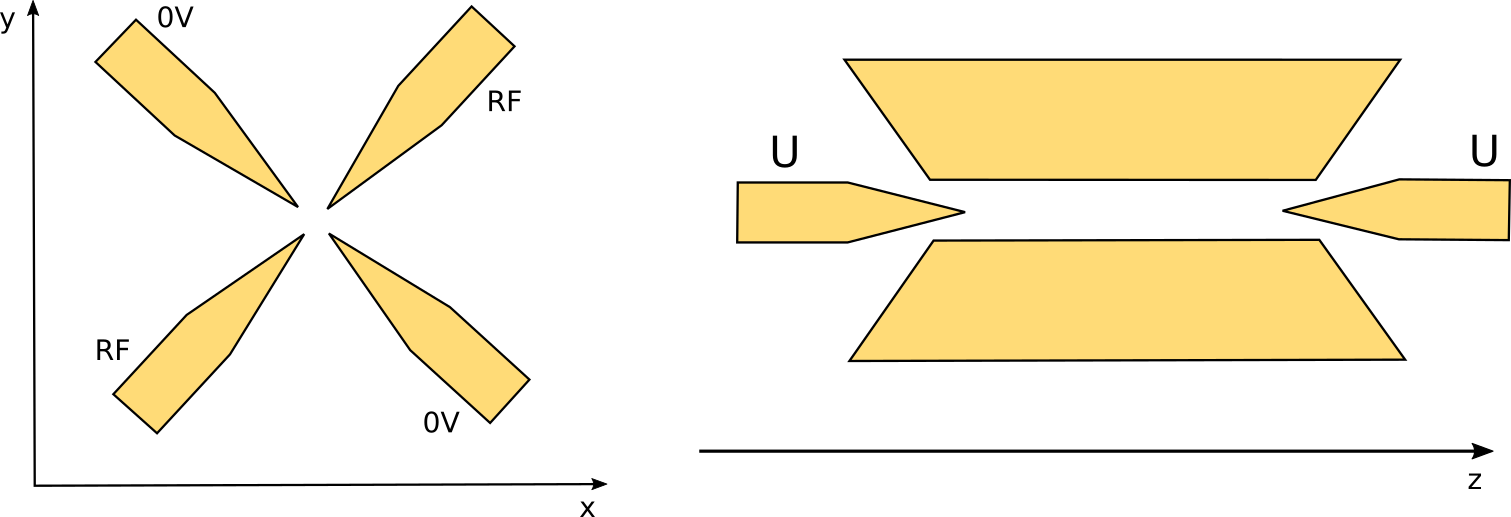
\includegraphics[width = .7\textwidth]{trap}
\caption{A linear paul trap. U is the voltage applied to the electrodes trapping in the $z$ direction, while in the $x-y$ plane trapping is achieved with a radio frequency signal.}
\label{trap}
\end{figure}
The confinement in the $x-y$ plane is provided by 4 electrodes, two of which are grounded and the other two are connected to a radio frequency source. This design is similar to a mass filter, with the difference of additional endcap electrodes in the $z$ direction that plug the trap and confine also in the axial direction.\par
The potential inside the trap can be described for the $x-y$ plane independently from the $z$ direction. In the case of a linear Paul trap the radial potential is \cite{traptheory}:
\begin{equation}
\phi  = \frac{\Phi_0}{2r_0^2}\left(x^2 - y^2\right),
\end{equation}
where $r_0$ is the distance from the center of the trap to the electrodes. The amplitude consists of a static part $U_0$ and a dynamical one $\Phi_0 = U_0 + V \cos(\Omega_{RF} t)$.
The study of the particle's motion with mass $m$ and charge $e$ inside the trap can be done with classical physics, Newton's second law in this case is
\begin{equation}
m\ddot{x} = -q \frac{\partial \phi}{\partial x} = - \frac{ex}{r_0^2}\left(U_0 + V \cos(\Omega_{RF} t) \right),
\end{equation}
and similarly for $\ddot{y}$. This equation can be written in the form of Mathieu equation \cite{Richards1983} by defining two parameters:
\begin{equation}
a_x = \frac{4eU_0}{\Omega_{RF}^2r_0^2m}, \quad q_x = \frac{2eV}{\Omega_{RF}^2r_0^2m} \implies \ddot{x} +\frac{\Omega_{RF}}{4} \left(a_x + 2q_x \cos(\Omega_{RF} t )\right)x = 0
\end{equation}
and with a change of variable $\tau = \frac{\Omega_{RF} t}{2}$ we end up with
\begin{equation}
\label{mathieu}
\frac{\partial^2 x}{\partial \tau^2}+\left(a_x + 2q_x \cos(2\tau)\right)x = 0
\end{equation}
This kind of equation has stable solutions that can be found in a recursive way with Floquet theorem \cite{iondynamic}. In the limit $a_x \ll q_x \ll 1$, solutions to \eqref{mathieu} are found to be
\begin{equation}
x(t) = x_0 \cos(\omega_x t +\phi_x)\left[1 + \frac{q_x}{2}\cos(\Omega_{RF} t) \right].
\end{equation}
Here, we recognize a oscillation $\omega_x$, referred to as \emph{secular motion}, with amplitude modulated by a oscillation $\Omega_{RF}$, called \emph{micromotion}. The approximation, named secular, is valid only in the case $\omega_x \ll \Omega_{RF}$. The frequency $\omega_x$ is given in the solution as
\begin{equation}
\label{eq:wx}
\omega_x = \frac{\Omega_{RF}}{2}\sqrt{a_x + \frac{q_x^2}{2}}.
\end{equation}
By imposing real solutions to \eqref{eq:wx}, the stability diagram of the trap can be found \cite{traptheory}. The other spatial dimension can be treated in the same way and the results are the same.\par
Confinement in the axial direction $z$ is purposely weaker, and ions will align in this direction. Two electrodes with constant potential $U$ are present, they create a harmonic potential
\begin{equation}
V = \frac{1}{2}m\omega_z^2z^2,
\end{equation}
where $\omega_z$ is the axial trap frequency. In the case of a string of ions, mutual repulsions must also be included, in the next section we will consider this case.

\subsection{Ion strings}
\label{ionstrings}
For the goals of this thesis, we are interested in the separation between $N$ ions loaded in the trap. This will give us an idea of how narrowly the beam should be focused and will set an appropriate problem spatial scale.\par
Let us consider the $z$ direction where the ions are more weakly confined such that they form a string. The potential can be approximated as harmonic and hence given by
\begin{equation}
V = \sum_{i=0}^N \frac{1}{2}m\omega_z^2z_i^2 + \sum_{i\neq j}^N\frac{Z^2e^2}{8\pi \epsilon_0}\frac{1}{|z_i-z_j|},
\end{equation}
where $z_i$ is the position of the $i-$th ion, and $Z$ the degree of ionization of the ions. The equilibrium positions can be found at the minima of the potential, i.e. where the first derivative zeros
\begin{equation}
\frac{\partial V}{\partial z_i} = 0 \implies u_i - \sum_{j=1}^{i-1} \frac{1}{(u_i-u_j)^2} + \sum_{j= i+1}^{N} \frac{1}{(u_i-u_j)^2}= 0,
\end{equation}
where we defined the dimensionless quantity $u_i = z_i/l$ and $l^3 = \displaystyle\frac{Z^2 e^2 }{4\pi \epsilon_0 m\omega^2}$.
The last equation can be solved analytically for 2 or 3 ions \cite{ion_spacing}. For the case $N=2$ we get the system
\begin{equation}
\begin{cases}
  u_1 + \frac{1}{(u_1-u_2)^2} = 0\\
  u_2 - \frac{1}{(u_1-u_2)^2} = 0
  \end{cases} \quad \implies \quad u_1 = -u_2,\quad  u_1 = \left(\frac{1}{2}\right)^{2/3} \simeq 0.629
\end{equation}
For $^{40}\text{Ca}^+$ ions (atomic mass $\simeq 40$ u \cite{AUDI2003337}) in a Paul trap with axial confinement of $\omega_z = 2\pi \times 1$ MHz, we have $l \simeq 4.4\times 10^{-6}\,$m, which means that 2 ions are separated by $\simeq 5.6\, \mu$m. This size is accessible since it is above diffraction limit (ref. Section \ref{sec_diffraction}) for optical atomic transitions.
In Figure \ref{positions_ions}, ions positions are presented for different number of ions $N$ trapped with an axial confinement of $\omega_z = 2\pi \times 1$ MHz.

\begin{figure}[H]
\centering
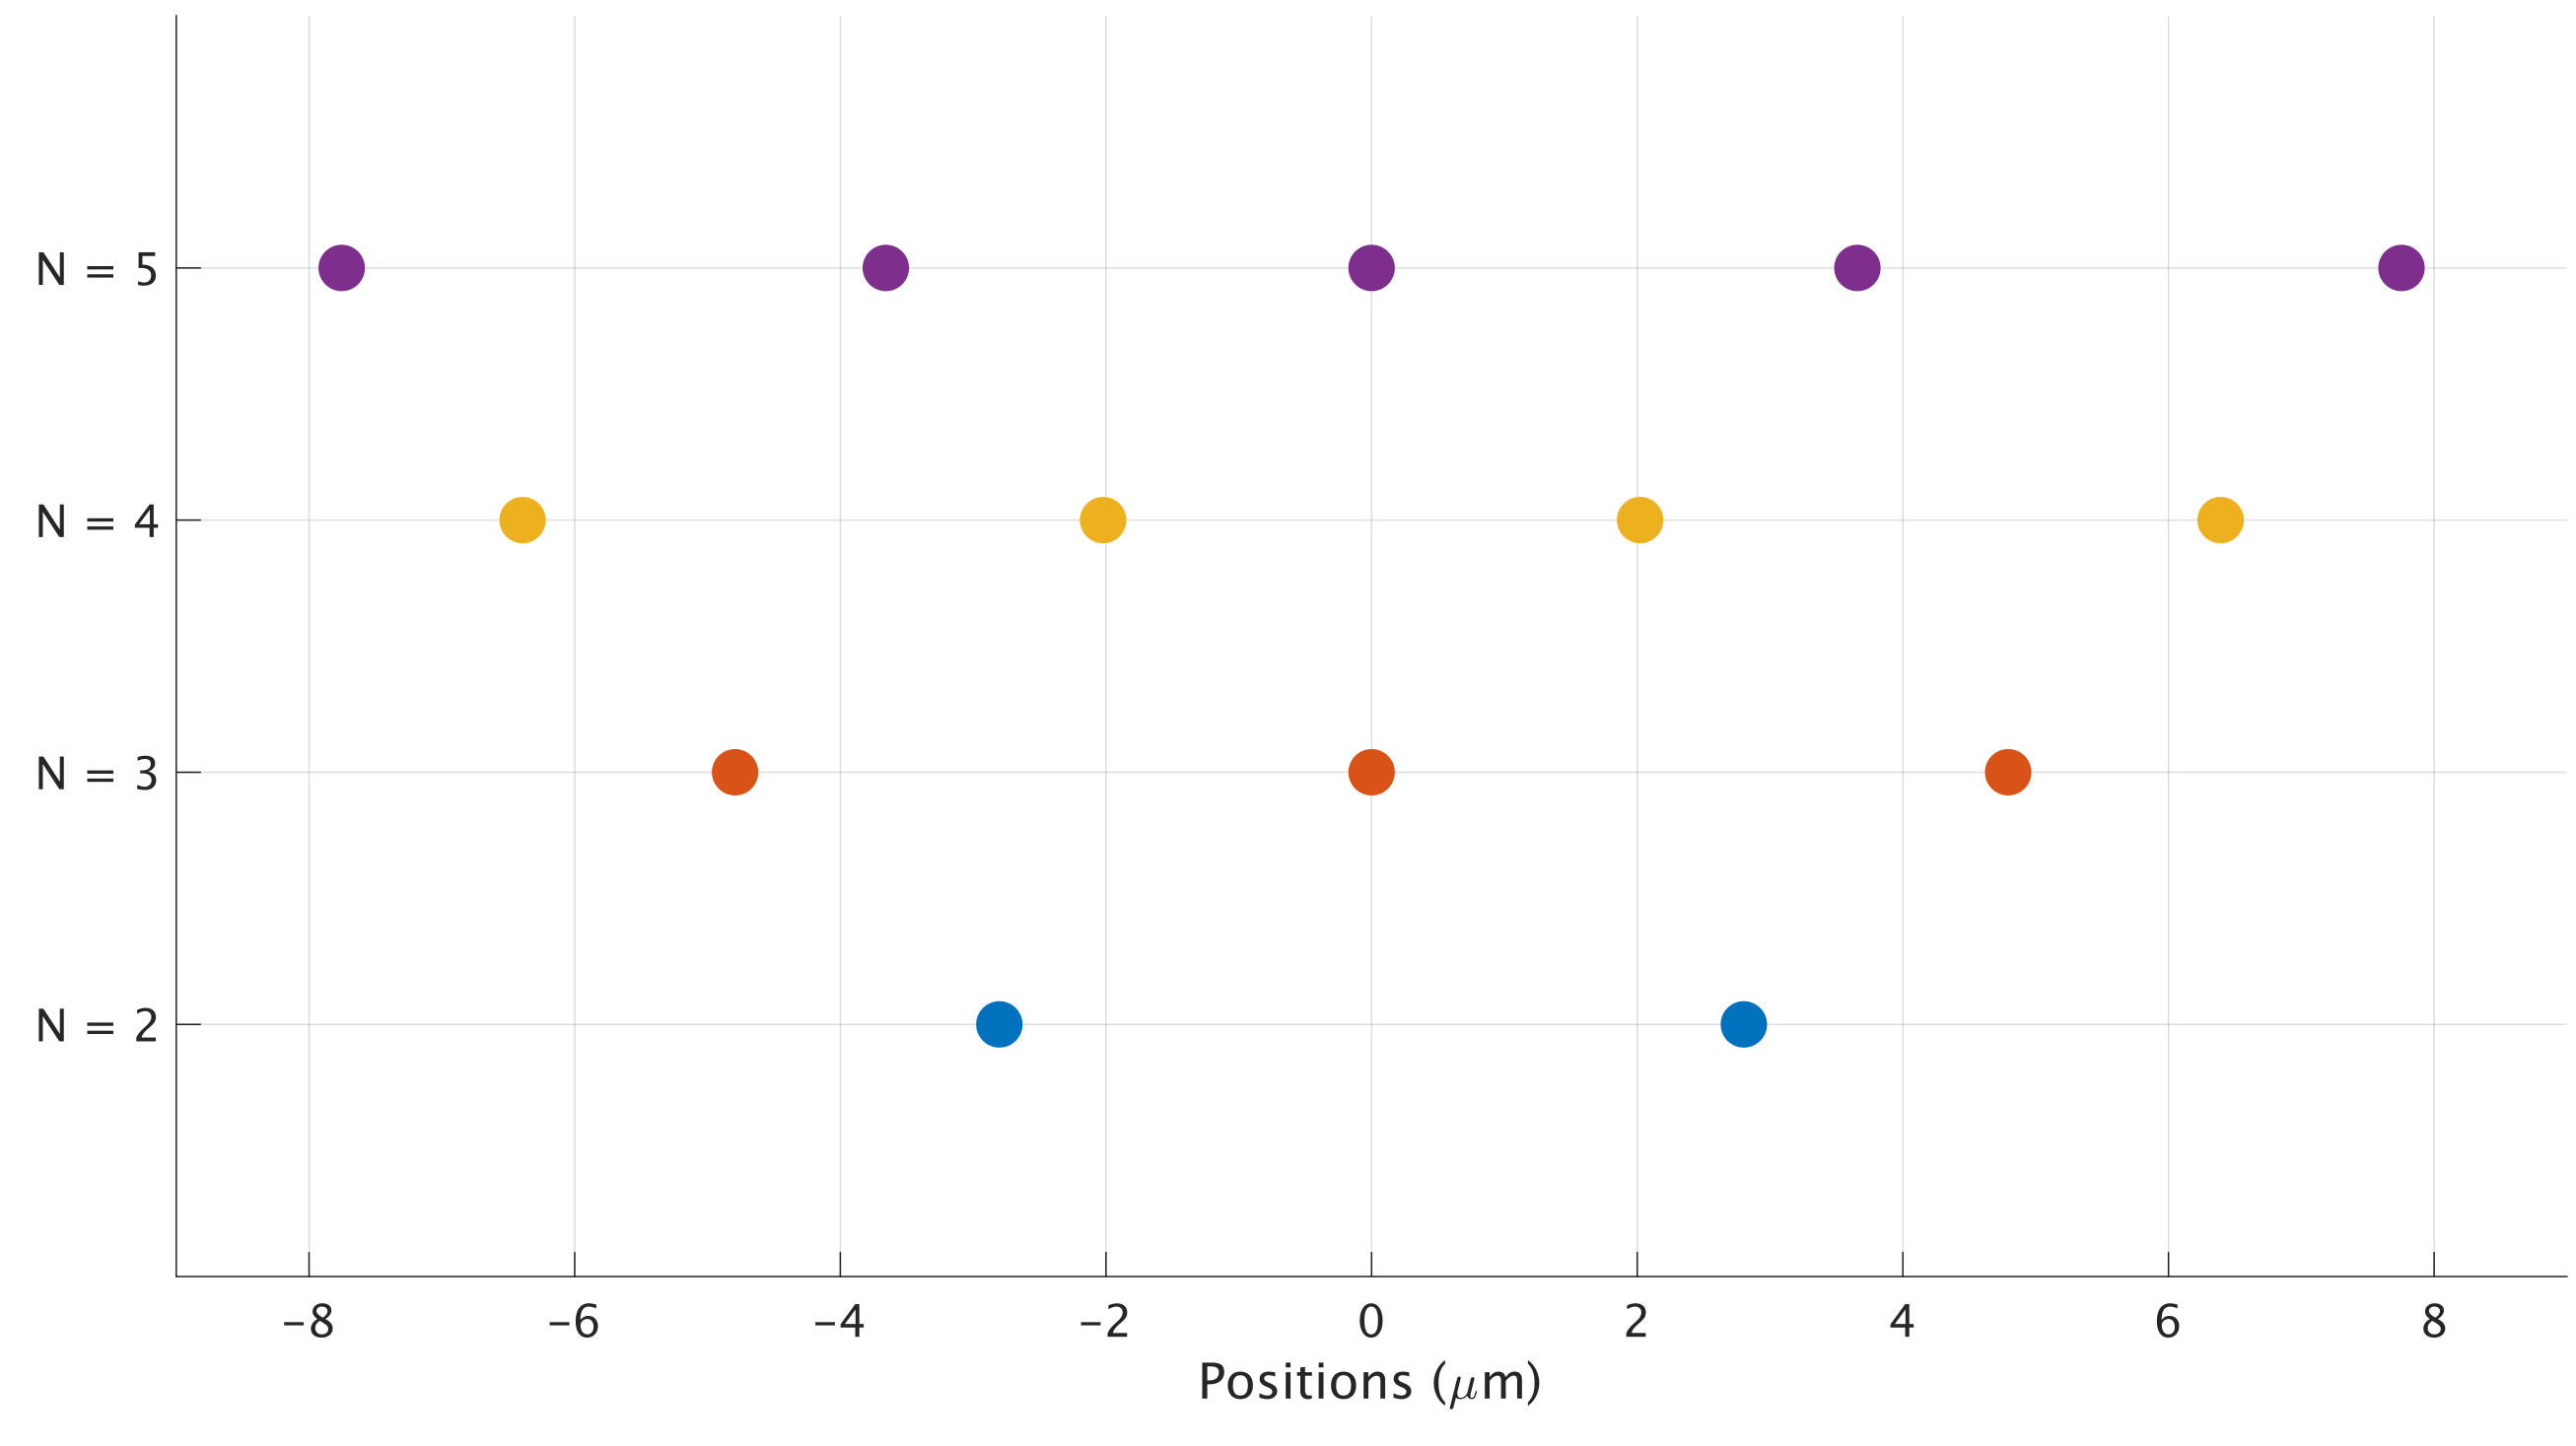
\includegraphics[width = \textwidth]{positions_ions2}
\caption{Ions position for different number $N$ of ions in the trap. Confinement is $\omega_z = 2\pi\times 1$ MHz.}
\label{positions_ions}
\end{figure}
%
%
% \begin{figure}[H]
% \centering
% 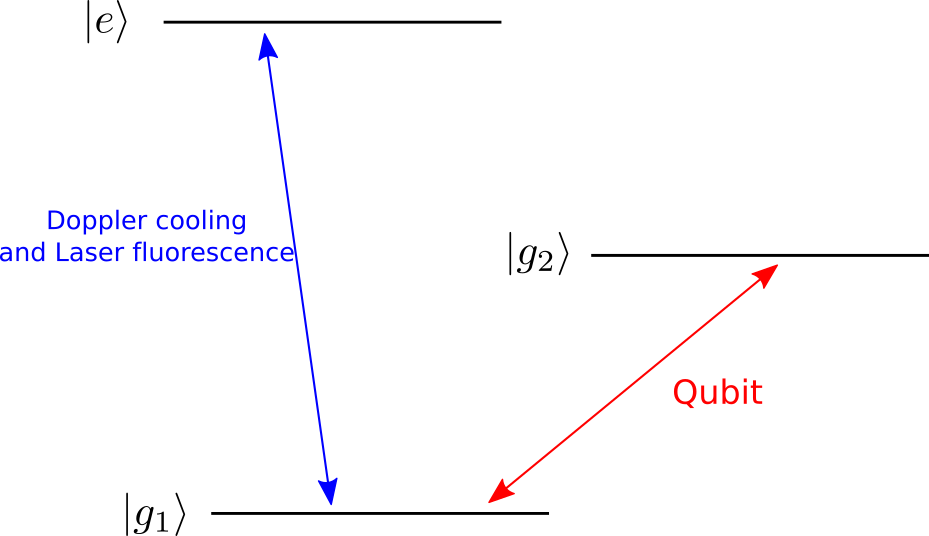
\includegraphics[width = .6\textwidth]{threelevelatom}
% \caption{$\Lambda$ type scheme. Two ground states $\ket{g_1}$ and $\ket{g_2}$ are stable or metastable, while the excited level $\ket{e}$ is short lived. Qubit is encoded in the two ground states while laser fluorescence and laser cooling is done on the $\ket{g_1}\to \ket{e}$ transition. The transition $\ket{e}\to \ket{g_2}$ is repumped to avoid for the electron to be stuck in $g_2$.}
% \label{threelevel}
% \end{figure}
\subsection{Doppler cooling}
\label{sec:doppler_cooling}

Coherent manipulation of ions requires cooling them to reach at least the Lamb Dicke regime \cite{Wineland1998}, where the extent of the ion wave packet is much smaller than the optical wavelengths of the lasers. The idea comes from neutral atoms \cite{1975OptCo..13...68H} and can be applied to ions as well: a laser interacts with a particular transition, causing photon absorption from the laser by the atom, giving a momentum kick $\Delta p = \hbar \mathbf{k}$ in the direction of the laser beam to the ion. The absorbed photon is emitted through spontaneous emission in a random direction, giving another kick to the ion. Over many cycles of absorption and emission, the random kick due to emission will average to zero (although presents a heating process which sets the Doppler limit), while the kick given by the laser will slow down and cooling the ion in the direction of the laser. \par
The mathematical model is a 2-level atom interacting with a laser (Rabi frequency $\Omega$, and detuning $\Delta$) as described in Section \ref{laserioninteractions}. Spontaneous emission is included with the master Equation \eqref{masterequation}, where $\Gamma$ is the spontaneous emission rate. The master equation can be explicitly written for every component of the density matrix $\rho_{ij}$, in the rotating frame they are called optical Bloch equations \cite{foot}. Following the approach of \cite{gabriel}, the system reaches equilibrium when $\rho_{ee}(t\to \infty)$:
% \begin{equation}
% \label{rhoee}
% \frac{d\rho_{ee}}{dt} = -i\frac{\Omega}{2}(\rho_{eg} - \rho_{ge}) - \Gamma \rho_{ee}
% \end{equation}
% \begin{equation}
% \frac{d\rho_{gg}}{dt} = i\frac{\Omega}{2}(\rho_{eg} - \rho_{ge}) + \Gamma \rho_{ee}
% \end{equation}
% \begin{equation}
% \frac{d\rho_{ge}}{dt} = -\left(\frac{\Gamma}{2}+i\Delta\right)\rho_{ge} -i\frac{\Omega}{2}(\rho_{ee} - \rho_{gg})
% \end{equation}
% \begin{equation}
% \frac{d\rho_{eg}}{dt} = -\left(\frac{\Gamma}{2}-i\Delta\right)\rho_{eg}+i\frac{\Omega}{2}(\rho_{ee} - \rho_{gg})
% \end{equation}
\begin{equation}
\rho_{ee}(t\to \infty) = \frac{\Omega^2/\Gamma^2}{1 + \left(2\frac{\Delta -\mathbf{k}\cdot \mathbf{v}}{\Gamma}\right)^2 + 2\frac{\Omega^2}{\Gamma^2}}
\end{equation}
where $\mathbf{v}$ the velocity of the ions. The force exerted on the ions, due to the radiative pressure, is proportional to $\rho_{ee}$ as
\begin{equation}
F = \hbar k \Gamma \rho_{ee} \simeq F_0 + \frac{dF}{dv}v = \hbar k \Gamma\frac{\Omega^2}{\Gamma^2 +4\Delta^2} + F_0 \frac{8k\Delta}{\Gamma^2 + 4\Delta^2}v
\end{equation}
where we assumed low velocities $v \simeq 0$ and thus linearized the equation. The effect of the constant term in the force is just to displace the ion from its central position. Instead, the linear term acts as a viscous friction that cools the ions with a rate of $\dot{E}_c = \braket{Fv}$.
If on one side spontaneous emission allows for Doppler cooling, it also sets the lower limit. The small fluctuations in the Brownian motion leads to diffusion which heats the ion at a rate of
\begin{equation}
\dot{E}_h = \frac{1}{m}\frac{d}{dt}\braket{p^2} =  \frac{1}{m}(\hbar k)^2 \Gamma \braket{\rho_{ee}(v)}.
\end{equation}
At equilibrium, the heating rate equals the cooling rate giving the lowest temperature achievable
\begin{equation}
\dot{E}_h + \dot{E}_c = 0  \implies k_B T = -\frac{\hbar \Gamma}{4}\left(\frac{\Gamma}{2\Delta} +\frac{2\Delta}{\Gamma}\right).
\end{equation}
From here it is clear that by choosing the appropriated detuning, it is possible to reach the lowest temperature
\begin{equation}
T_{min} = \frac{\hbar \Gamma}{2k_{B}}, \qquad \text{for} \quad \Delta = -\frac{\Gamma}{2}.
\end{equation}
At this temperature, the average phonon number is $\braket{\hat{n}} = \Gamma /2\omega_z$ \cite{Eschner:03}.\par
As an example, a single calcium ion confined in a trap with $\omega_z = 2\pi\times 1$ MHz, can be cooled using the transition $\ket{\text{S}_{1/2}}\to \ket{\text{P}_{1/2}}$ ($\Gamma = 2\pi\times 20.8$ MHz), the 2-level atom model in this case gives a good estimation, even though calcium has more levels. The Doppler temperature is $T_{min} \sim 500\,\mu$K, and the corresponding average phonon number is $\braket{\hat{n}} = 10.4$. The wavefunction extent for this phonon number can be found as the standard deviation of the operator $\hat{z}$ for the vibrational state $\ket{n}$
\begin{equation}
\sigma_z = \sqrt{\braket{\hat{z}^2}} = \sqrt{\frac{\hbar}{2m\omega_z}(1+2\braket{\hat{n}})} \simeq 52\,\text{nm}.
\end{equation}
Such a Doppler cooled ion has therefore a spatial dimension still much smaller than the ion separations and the wavelength of the relevant lasers.\par
To further decrease $\braket{\hat{n}}$, sideband cooling can be used \cite{Eschner:03}, here particular sideband transitions are excited to reduce the phonon number of the ions inside the trap. However in the experiments of this thesis, only Doppler cooling has been performed.
\section{Laser beam}
\subsection{Gaussian beams}
\label{sec_diffraction}
Typically, lasers emit light in the shape of Gaussian beams, so it is import to understand what Gaussian beams are and their characteristics. In this chapter we will take a closer look into such beams and introduce important quantities to characterize a Gaussian beam. \par
From a theoretical point of view, Gaussian beams are a solution of the Helmholtz equation $(\nabla^2 + k^2)U(\mathbf{r}) = 0$, with $k$ being the wavevector, and $U(\mathbf{r})$ the complex electric field. If we can consider a wave propagating in the $z$ direction, we can write $U(\mathbf{r})$ as \cite{saleh}:
\begin{equation}
\label{gaussianbeams}
U(\mathbf{r}) = A_0 \frac{W_0}{W(z)}\exp\left\{-\frac{x^2+y^2}{W^2(z)}\right\}\exp\left\{-ikz-ik\frac{x^2+y^2}{2R(z)}+i\arctan(z/z_0)\right\}.
\end{equation}
Where $A_0$ is an amplitude, $W(z)$ the width, $R(z)$ the curvature radius, and $z_0$ the Rayleigh range. The intensity can be calculated by taking the square of the complex amplitude
\begin{equation}
\label{beamintensity}
I(\mathbf{r}) = |U(\mathbf{r})|^2 = I_0 \left(\frac{W_0}{W(z)}\right)^2 \exp\left\{-\frac{2x^2 + 2y^2}{W^2(z)}\right\}  \qquad I_0 = |A_0|^2.
\end{equation}
For a fixed $z$, the sections in the $x-y$ plane are shaped as a two dimensional Gaussian distribution. For simplicity, let us take the profile for a fixed $z$ and $y=0$:
\begin{equation}
I(x,y=0,z) = \widetilde{A}(z) \exp\left\{\frac{2x^2}{W^2(z)}\right\} \qquad \widetilde{A}(z) = I_0 \left(\frac{W_0}{W(z)}\right)^2  .
\end{equation}
In Figure \ref{gauss}, the $x$ cross section is depicted for this intensity profile normalized in amplitude. Parameters used to measure the width are also displayed and defined in the caption. All of those quantities are equivalent and differ only by a prefactor, so for the rest of the section, we stick to $W(z)$ (point at which $I$ has fallen to $1/e^2 = 13.5\%$) and study its behaviour.
\begin{figure}
\centering
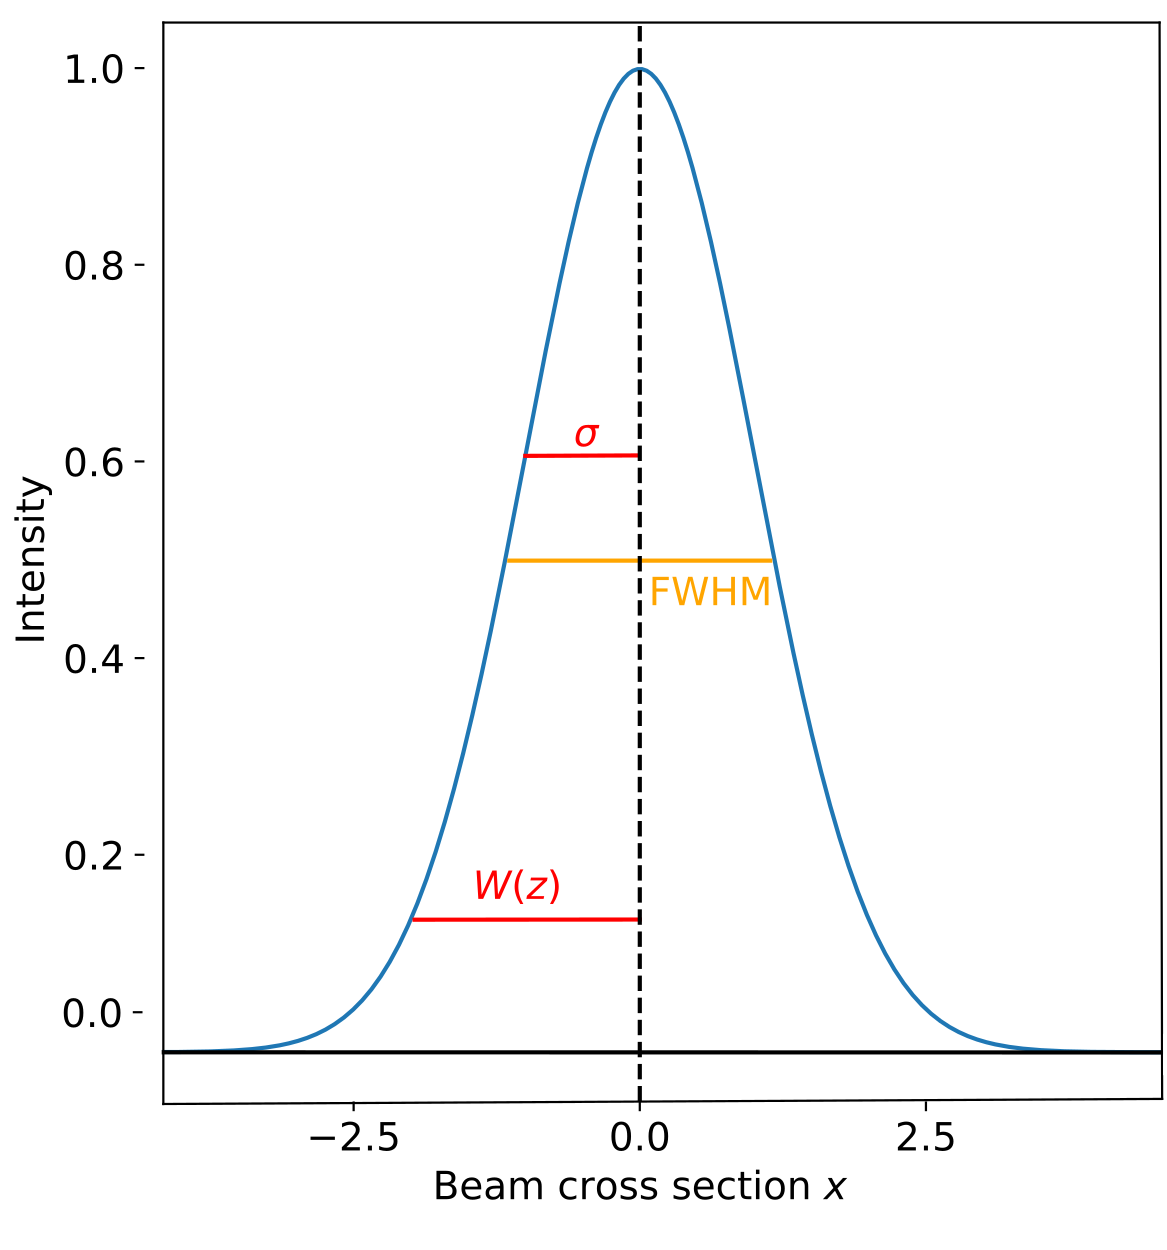
\includegraphics[width = .6\textwidth]{gauss2}
\caption{Cross section of the intensity profile of a Gaussian beam $I(x) = e^{-x^2/2\sigma^2}$. The beam is normalized and $\sigma=1$. Graphical representations of used widths are displayed: $W(z)$ is defined as the point at which the intensity $I$ has fallen to $1/e^2 = 13.5\%$ of its maximum value; $\sigma$ is the standard deviation of a Gaussian in the form $Ae^{-\frac{x^2}{2\sigma^2}}$; FWHM is the full width half maximum. Relationships among these quantities are: $W(z) = 2\sigma$, and $W = 0.84\cdot \text{FWHM}$.}
\label{gauss}
\end{figure}
From Helmholtz equation \cite{saleh}, the profile of $W(z)$ as a function of $z$ is found to be
\begin{equation}
\label{waistprofile}
W(z) = W_0 \sqrt{1 + \left(\frac{z}{z_0}\right)^2}\qquad W_0 = \sqrt{\frac{\lambda z_0}{\pi}} \qquad z_0 = \frac{\pi W_0^2}{\lambda}.
\end{equation}
$\lambda$ is the wavelength, and $W_0$ and $z_0$ are respectively the waist of the beam and the Rayleigh range discussed below. A plot of Equation \eqref{waistprofile} is presented in Figure \eqref{gaussprofile}:
the width $W(z)$ assumes its minimum value $W_0$ at $z=0$, this position is called the beam focus and its width $W_0$ is the waist of the beam. The Rayleigh range $z_0$ gives an idea of how quickly the beam is expanding. Mathematically, $z_0$ is the distance between the focus and the point where the width is $W(z) = \sqrt{2}W_0$.
For $z \gg z_0$, the beam profile diverges almost linearly with an angle given by $\theta = W_0/z_0$, which means the smaller the focus, the greater it diverges.\par
This property will become important later in the work, because it provides one limit on the waist of the beam in our experimental system. The optical aperture of the trap is limited by some electrodes, and a beam that diverges too rapidly can potentially clip on one electrode causing aberrations and scattered light in the trap.\par
A Gaussian beam can be reshaped using optical elements.
\begin{figure}
\centering
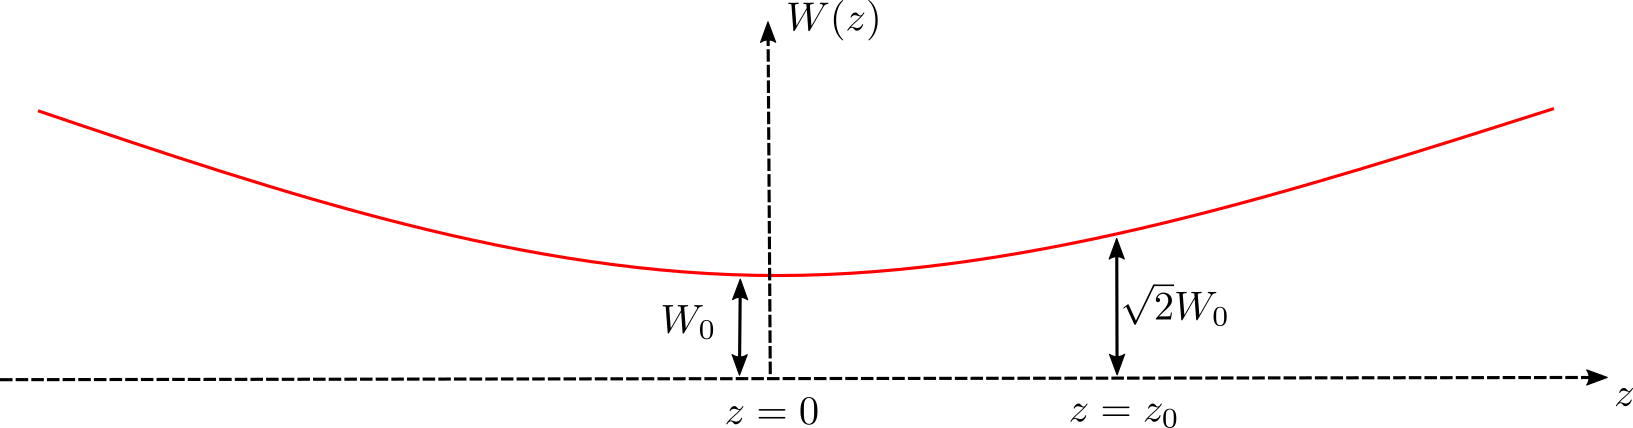
\includegraphics[width = \textwidth]{gaussprofile}
\caption{Width profile of a Gaussian beam along the direction of travel of the beam, Equation \eqref{waistprofile}. The beam is focused at the position $z = 0$, here it assumes the minimum width $W_0$, also referred to as the waist. $z_0$ is the Rayleigh range where the width is $\sqrt{2}W_0$}
\label{gaussprofile}
\end{figure}
In order to study such reshaping, let us consider a thin spherical lens with focal length $f$ placed at position $z$. The effect of the lens on the beam is to give an extra phase factor $k(x^2 + y^2)/2f$ to Equation \eqref{gaussianbeams} \cite{beamparameters}. We can match the phase of the incoming and emerging waves, which have respectively radius of curvature $R$, and $R'$, this results in
\begin{equation}
\frac{1}{R'} = \frac{1}{R} - \frac{1}{f}.
\end{equation}
The effect of the lens is to change the radius of curvature to $R'$. Moreover, the width of the beam at the lens is not altered $W=W'$. Using these last two facts, we can determine all the parameters of the outgoing wave. The most important for us is the new waist $W_0'$
\begin{equation}
W_0' = MW_0 \qquad M = \frac{M_r}{\sqrt{1+r^2}}.
\end{equation}
Where $M_r = \left|\frac{f}{z-f}\right|$, and $r = \frac{z_0}{z-f}$. $M$ is the magnification factor which provides an easy way to describe the change of the beam. For a better understanding of this last result, let us consider a less general example. We place the lens at the focus $z=0$, and have a collimated beam $z_0 \to +\infty $. In this case the new waist is
\begin{equation}
\label{eq:newwaist}
W_0' = \frac{W_0}{\sqrt{1 + (z_0/f)^2}} \simeq W_0\frac{f}{z_0} = \frac{\lambda f}{\pi W_0}
\end{equation}
where the approximation comes from taking $z_0\gg f$. There are three parameters we can act on to achieve the smallest waist. A shorter wavelength $\lambda$ results in a smaller waist. Similarly, a lens with a shorter focal length $f$ reduces the waist. Finally, a broader incoming beam, i.e. larger $W_0$, also narrows the waist. Given a certain lens and a wavelength, the smallest waist is obtained with the largest incoming beam which is limited by the lens diameter $D$, i.e. $2W_0 = D$. In this case, equation \ref{eq:newwaist} becomes
\begin{equation}
\label{eq:difflimited}
W_0' = \frac{2\lambda}{\pi} \frac{f}{D}.
\end{equation}
If the size of the collimated beam is further increased, the lens becomes a finite size aperture and diffraction effects will appear at the image plane. In general, an optical system (in our example a single lens) that is limited in the sense of \eqref{eq:difflimited} is said to be diffraction limited \cite{diocane}.
%An a numerical example, the objective used in this thesis setup has an aperture of 40 mm, focal length of 54 mm, therefore for a wavelength of $\lambda = 393$ nm the best achievable waist is $1.02\,\mu$m.

\subsection{Beam stearing via Acousto-optical Deflectors}
\label{theory_AOD}
An acousto-optical deflector (AOD) is a common device that can change the propagation direction of a laser beam, typically on the few microsecond timescale. In this work we use an AOD to change which ion is illuminated by a single-ion focused laser. The working principle of an AOD is based on the Acousto-optical effect. A piezo is used to create acoustic waves that propagate through a crystal. The waves modify the crystal refractive index, creating a periodic optical grating that can deflect light travelling through it.  \par
Following the approach of \cite{saleh} to model the device, let us consider a rectangular crystal like in Figure \ref{AOD}. The acoustic wave creates a sinusoidal pattern with frequency $\Omega_s$ and wavenumber $q$, for the refractive index $n(x,t)$
\begin{equation}
n(x,t) = n - \Delta n_0 \cos \left(\Omega_s t - qx \right),
\end{equation}
where $n$ is the refractive index of the unperturbed medium, $\Delta n_0$ is the amplitude of the perturbation. $\Delta n_0$ is proportional to the square root of the sound intensity.
\begin{figure}
\centering
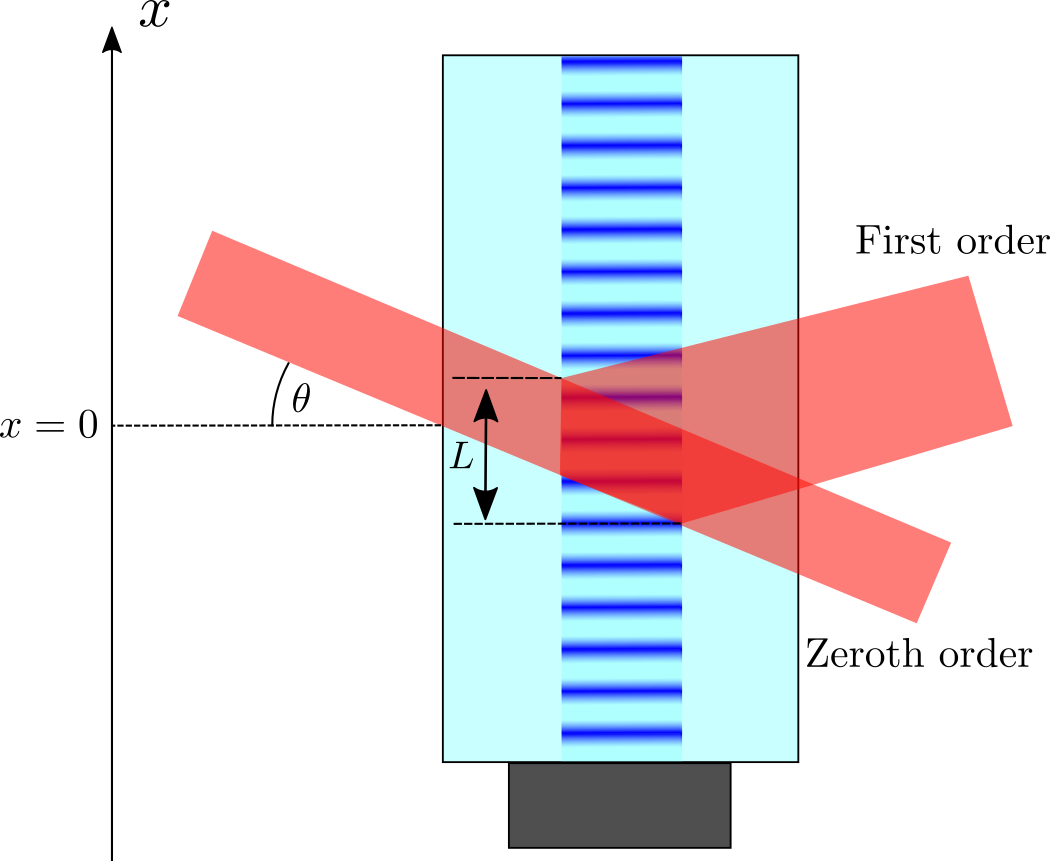
\includegraphics[width = .5\textwidth]{aod3}
\caption{Simple model of an AOD. In black at the bottom a black piezo that generates acoustic waves through the light blue crystal. In red, a collimated beam of light enters in the crystal with an angle $\theta$ and gets partially deflected at an a angle $\theta_d$ due to the interaction with the effective optical grating created by the acoustic waves. $L$ is the interaction length.}
\label{AOD}
\end{figure}
The refraction\footnote{defined as $E_r/E_i = r$, where $E_r$ is the refracted electric field, and $E_i$ is the input field} $r$ can be calculated by dividing the crystal in thin layers with thickness small compared to the acoustic wavelength. We assume that the refractive index $n(x)$ is approximately constant across the layer. The total refraction is given by all the contributions $dr/dx$ of every layer, we can therefore integrate in the $x$ direction over the length $L$ (see Figure \ref{AOD}) as follows:
\begin{equation}
r = \int_{L/2}^{L/2} e^{i2kx \sin\theta} \frac{dr}{dx} \,dx
\end{equation}
The included phase $e^{i2kx \sin\theta}$ takes into consideration the different phase of the input laser beam when different layers are met. The integral can be solved with a change of variable $dr/dx = q \Delta n_0 \sin \left(\Omega_s t - qx \right)dr/dn $. The sine function can be written as exponential and now the integral contains only exponential functions which are straightforward to calculate. At the end we obtain two contributions for the refracted wave $r$:
\begin{equation}
\label{mainAOD}
r = r_+ + r_- \qquad r_\pm = \pm i r_0 \text{sinc} \left[(2k\sin(\theta) \mp q)\frac{L}{2\pi} \right]e^{\pm i\Omega_s t}
\end{equation}
These two terms are the plus and minus first order diffraction, an acousto-optical device can be operated symmetrically entering either with a positive angle or with a negative one. Since the maths and the physics is the same, we will focus only on the positive term, called upshifted Bragg diffraction. The sinc function peaks sharply when its argument is 0, i.e. at $2k\sin\theta = q$, and then quickly decreases as the angle is changed. Hence, the input beam must enter with a particular angle $\theta_B$ in order to diffract with maximum efficiency. The condition to be satisfied is called the Bragg condition, and can be written as a function of the optical ($\lambda$) and acoustic ($\Lambda_s$) wavelengths as
\begin{equation}
\label{braggcondition}
\sin \theta_B  = \frac{\lambda}{2 \Lambda_s} \qquad \Lambda_s = \frac{2\pi}{q}.
\end{equation}
At the Bragg angle, the diffraction angle $\theta_d$ is equal to the incident angle $\theta_B = \theta = \theta_d$ \cite{Korpel1981}. If the condition is not perfectly matched, some light will not be diffracted and will be transmitted unaltered through the device. The ratio of the transmitted and diffracted light is called diffraction efficiency and gives an idea of how well an acousto-optical device is performing.\par
From Equation \eqref{mainAOD} we can notice that an extra phase factor proportional to $\Omega_s t$ is added to the reflected wave. Thus, if the incoming wave is oscillating at $\propto e^{i\omega t}$, the diffracted wave will oscillate as $\propto r_{+}e^{i\omega t} \implies \propto e^{i(\omega + \Omega_s )t}$. The frequency of the diffracted optical wave $\omega_r$ is therefore shifted by the frequency of the acoustic vibration as
\begin{equation}
\label{eq:aodshift}
\omega_r  =  \omega + \Omega_s.
\end{equation}
The acousto-optical effect described above is common to different devices optimized for specific tasks. Two of the most commons devices are Acousto-optical Deflectors (AOD) and Acousto-optical Modulators (AOM). The idea of the latter is to shift the frequency of a laser using Equation \eqref{eq:aodshift}. Deflectors instead aim to shift the direction of the beam by exploiting the fact that the diffraction angle $\theta_d = \theta$ changes linearly as a function of the acoustic frequency $\Omega_s$. Assuming that the angle $\theta$ is small enough to approximate $\sin\theta \sim \theta$, the Bragg condition can be written as
\begin{equation}
\label{eq:deflection}
\theta \simeq \frac{\lambda}{2 v_s}f,
\end{equation}
where $v_s$ is the speed of sound and $f$ the frequency of the acoustic wave. We can already see that if we change the frequency $f$, the deflection angle $\theta$ changes proportionally. The bandwidth $B$ specifies the range of frequencies over which deflectors work. Assuming that the maximum diffraction angle is $\Delta\theta$, Equation \eqref{eq:deflection} can we written as \cite{Rmer2014}
\begin{equation}
\label{eq:deflection}
\Delta\theta \simeq \frac{\lambda}{2 v_s}B,
\end{equation}
It is clear from this equation that, in order to increase the bandwidth, i.e. increasing $\Delta \theta$, slower acoustic velocities are preferred. AODs are therefore optimized by choosing a crystal and an acoustic mode with low acoustic velocities compared to AOMs \cite{handbookoptics}.%\cite{handbookoptics}.

\section{Basic model of key experiments}
To fulfill the goals of this thesis we perform two key experiments with ions: single-ion qubit manipulation and single-ion photon generation. This section presents a short overview of those key experiments, using the theory introduced in the previous sections.

\subsection{Addressed qubit manipulation}
\label{sec:expqubit}
\begin{figure}
\centering
\includegraphics[width=.7\textwidth]{exp1}
\caption{a) Relevant levels for the experiment, the qubit is encoded in the 729 nm transition, the 393 nm laser is used to shift the $\ket{S}$ level via AC Stark shift b) Experiment pulse sequence, Doppler cooling and state readout are described in Section \ref{sec:expparameters}. The time $\tau$ had a variable length.}
\label{img:qualcosa}
\end{figure}
As highlighted in Figure \ref{img:qualcosa}, the qubit is encoded in the $\ket{S}$ and $\ket{D}$ states. The 393 nm transition from $\ket{S}\to \ket{P}$ can be used to induce a phase shift on the ground state of the qubit $\ket{S}$. In the off resonant regime, the laser induces a AC Stark shift $\delta = \Omega^2/4\Delta$ (see Section \ref{laserioninteractions}) on the $\ket{S}$ and $\ket{P}$ states with negligible excitation of the $\ket{P}$ state. The effect of such AC Stark shift on the qubit is to shift the relative phase between $\ket{S}$ and $\ket{D}$ as shown below. As discussed in Section \ref{sec:dissipation}, in order to reduce spontaneous scattering in comparison to AC Stark shift, we should have $\delta \gg \Gamma_{eff}$. Therefore in the experiment we decided to set the detuning such that the ratio between the Stark shift and the spontaneous scattering rate is 100
\begin{equation}
\frac{\delta}{\Gamma_{eff}} = \frac{2\Delta}{\Gamma} \sim 100 \implies \Delta \sim 3\,\text{GHz}.
\end{equation}
\par Ion qubits can be used as sensitive tools for beam profiling. By measuring the state of all ion qubits individually, and scanning the beam across the ions string, a beam profile can be obtained. In a single experiment we can therefore characterize the beam and demonstrate qubit manipulation.
Specifically, the experiment performed is called Ramsey interferometry \cite{Ramsey1950}. In summary, the qubit begins in the $\ket{S}$ state, then the idea is to send a resonant $\pi/2$ pulse at 729 nm, which brings the qubit state to a superposition $\ket{S}+\ket{D}$, a second identical pulse would bring the final state to the excited level $\ket{D}$. However, if between the two 729 nm pulses, an AC stark shift is induced by a pulse of 393 nm light, an additional phase is added to the superposition. The phase of the second $\pi/2$ pulse is left as a variable to be scanned, as considered below. Rigorous mathematics can be done with matrices $U_{729}$ (Equation \eqref{laserpulse}) and $U_{393}$ (Equation \eqref{acstarkrotation}). After the three pulse sequence the final state is
\begin{equation}
\begin{split}
\ket{\psi_f} &= U_{729}(\pi,\phi)U_{393}(\delta)U_{729}(\pi,0)\ket{S} \\
&= \frac{1}{2}\left(e^{-i\frac{\delta}{2}\tau}-e^{-i\phi}\right)\ket{S}-\frac{i}{2}\left(1 + e^{-i\frac{\delta}{2}\tau} e^{-i\phi}\right)\ket{D}
\end{split}
\end{equation}
where $\delta = \Omega^2/4\Delta$ is the Stark shift, and $\Omega$ is the Rabi frequency of the 393 nm light that we want to measure. The final probability is then
\begin{equation}
\label{stupidequation}
P_D = \cos^2\left(2\phi + 2\frac{\delta \tau}{2}\right) = \cos^2\left(2\phi + \frac{\Omega^2 \tau}{4\Delta}\right).
\end{equation}
As we can see, $P_D$ depends on the phase of the second 729 nm pulse $\phi$ and on the Stark shift induced by the 393 nm laser. To get $\Omega^2$ a simple formula inversion can be done
\begin{equation}
\label{eq:ptointensity}
\Omega^2 = \frac{4\Delta}{\tau}\left[\text{arccos}\left(\sqrt{P_D}\right)-2\phi \right].
\end{equation}
The phase $\phi$ can be set experimentally.

\subsection{Addressed photon generation}
\label{sec:expphoton}
\begin{figure}
\centering
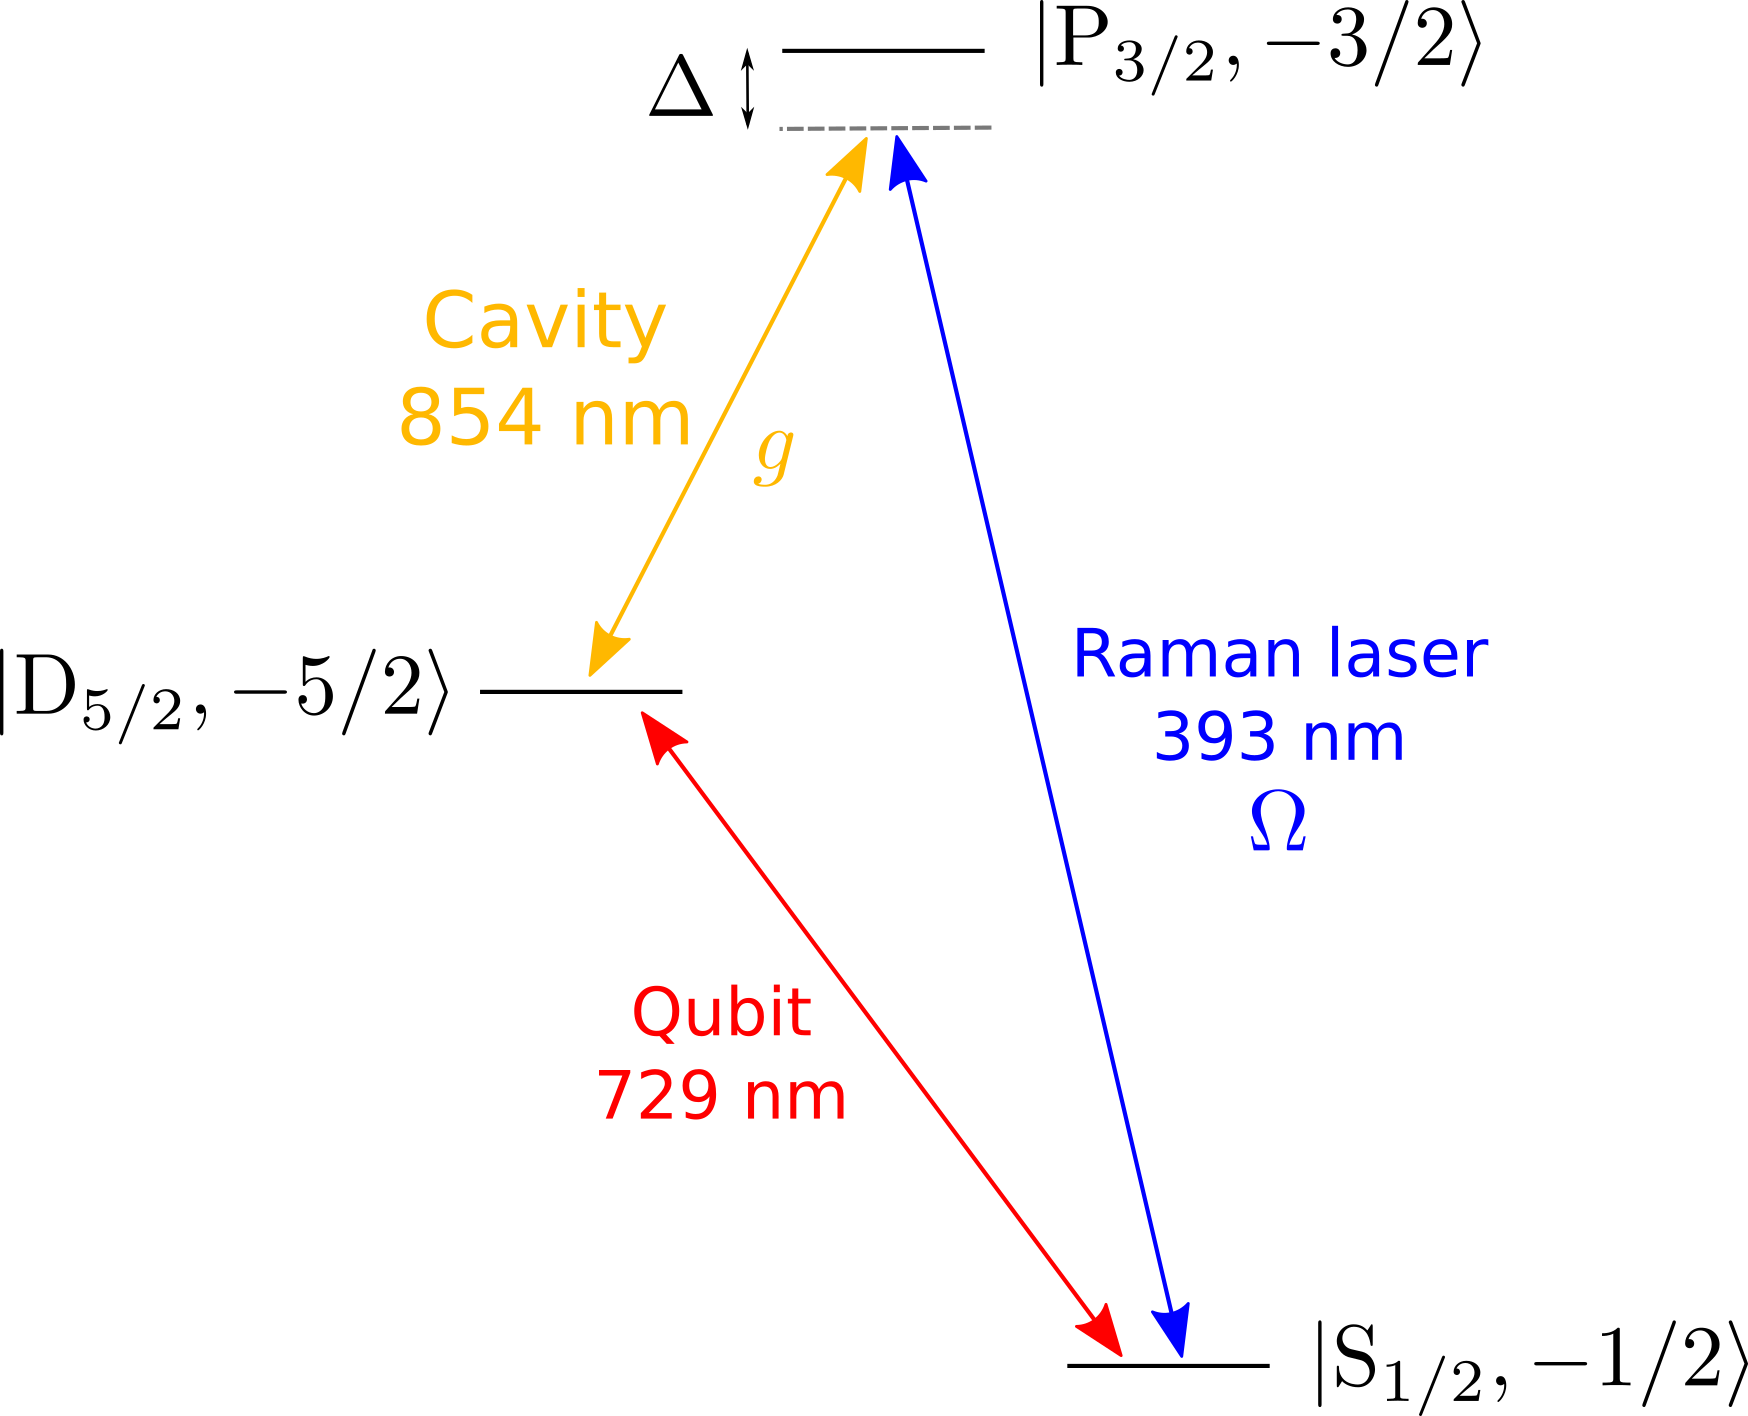
\includegraphics[width=.5\textwidth]{exp2}
\caption{Scheme of the Raman process used to generate photons, via a cavity enhanced Raman process (Section \ref{sec:ramanprocess}). The electron in the $\ket{S}$ state is excited to the $\ket{D}$ level by absorbing a 393 nm photon and emitting a 854 nm photon in the cavity.}
\label{img:sec2}
\end{figure}
The second key experiment consists of generating photons from one ion out of a string, using the cavity-mediated Raman process described in Section \ref{sec:ramanprocess}. In Figure \ref{img:sec2} the relevant levels are depicted. First, the ion is positioned in a maximum of the cavity vacuum electric field such that the atom-cavity coupling $g$ is maximized. Second, a 393 nm laser pulse triggers the generation of a photon into the cavity through the Raman process. As seen in Section \ref{sec:ramanprocess}, for the process to be stronger than the spontaneous scattering rate, we choose a detuning of $\Delta \sim 400$ MHz. In this case, the effective Rabi frequency $\Omega_{eff}$ (Equation \eqref{omegaeff}) is larger than the effective spontaneous scattering rate $\Gamma_{eff}$ (Equation \eqref{gammaeff}).\par
In the ideal case with finite probability, the population of the state $\ket{S}$ is coherently transferred to the $\ket{D}$ state by absorbing a 393 nm photon and emitting an 854 nm photon in the cavity, the photon then exits from the cavity out of a preferred mirror. We perform the experiment using the following states
\begin{equation}
\ket{\text{S}_{1/2},-1/2} \to \ket{\text{P}_{3/2},-3/2} \to \ket{\text{D}_{5/2},-3/2}.
\end{equation}
These transitions are polarization dependent, the absorbed photon is $\sigma_-$ polarized, while a $\pi$ polarized photon is emitted. Since the magnetic field is orthogonal to the cavity, the $\pi$ polarized photon is projected into a linearly polarized cavity photon.\par
Note that the effective Rabi frequency of the population transfer is proportional to the laser drive Rabi frequency $\Omega$ as seen in Equation \eqref{omegaeff}. On the contrary, the AC Stark shift depends on the Intensity $\Omega^2$. Therefore, the interaction of the addressed beam with the ion string in the two experiments is different. After the excitation and emission, qubit state detection on all ions is performed, this gives the possibility to check if other ions have been undesirably addressed.
